%!TEX root = ../thesis.tex
%*******************************************************************************
%****************************** FOURTH Chapter **********************************
%*******************************************************************************
\chapter{High-redshift Candidates}\label{chapter:high_redshift_candidates}

% **************************** Define Graphics Path **************************


\ifpdf
    \graphicspath{{Chapter4/Figs/Raster/}{Chapter4/Figs/PDF/}{Chapter4/Figs/}}
\else
    \graphicspath{{Chapter4/Figs/Vector/}{Chapter4/Figs/}}
\fi




\section{Motivation}\label{section:motivation_high_z}
The previous chapter concentrated on the task of optimising photometric redshift estimates for the \DESVIDEO catalogue, focused especially on optimal results at high redshifts. Furthermore, it also proposed a method for separating stars and galaxies based on the best-fit stellar and galaxy SEDs obtained during the photo-z computation. Together, these results
can be used to identify a collection of $z\gtrsim 5$ high-redshift candidates. The current chapter now describes the process of isolating such a sample. The purpose of this research is to investigate an optimal selection strategy, and to select a preliminary collection of high-redshift candidates. In future work, such a sample could be used to constrain the properties of galaxies in the early stages of evolution. Examples of such properties have been outlined in the introduction (see Section \ref{subsubsection:high_redshift_galaxy_evolution}). \par 

Although a strategy based on photometric redshifts could in principle retrieve any high-redshift galaxy with magnitudes brighter than the \DESVIDEO depths, the high photometric errors of objects close to the survey's limiting magnitude can lead to uncertain redshift estimates. To make sure redshifts for the candidate sample are maximally secure, this thesis concentrates on galaxies with $i$-band or $z$-band magnitudes below $m_{\mathrm{AB}}< 25$. These bright sources are particularly interesting, because as explained in Section \ref{subsubsection:lyman_break_galaxy_history}, the known samples of such objects are currently small. Section \ref{subsection:conclusion_high_z_intro} made the case how, thanks to the unprecedented size of a deep search area in the \DESVIDEO catalogue, the current work can thus provide a substantial increase in potential candidates. \par 

Moreover, this thesis focuses predominantly on Lyman-break galaxies, which are most likely to dominate  high-redshift samples. Despite the fact that a selection method based on photo-zs can theoretically also recover sources of other spectral types (provided these are represented in the template set), such objects are expected to be much less bright in the rest-frame UV (observed-frame optical), so they are unlikely to satisfy the brightness criteria. Furthermore, their spectral features  are much less distinct in the optical to near-IR wavebands, which makes them almost impossible to separate from stars or red low-redshift contaminants. For all the reasons listed above, the targets in this thesis thus consist of \textit{bright Lyman-break galaxies}. \par 


\section{High-redshift galaxy candidate selection process}\label{section:selection_criteria}
\subsection{Brief overview}\label{subsection:brief_overview}
After a careful investigation of possible selection criteria for high-redshift sources, the eventual strategy that was settled on consists of multiple stages. The task of the current part of this chapter is to describe this procedure. In order to clarify the structure of the upcoming discourse, a brief summary is listed below.  \par 

\begin{itemize}[leftmargin=4em]
    \item[\bf Step 1] The first stage is made up of a series of broad initial cuts, which are presented in Section \ref{subsection:broad_cuts}. The aim of this round is to extract a preliminary sample of bright high-redshift galaxy candidates. 
    \item[\bf Step 2] The next stage then involves visual examination of the preliminary candidates. Each object is assessed individually by looking at its imaging, photometry, and best-fit SEDs. Section \ref{subsection:visual_inspection} reports on this inspection, which has uncovered several major sources of contamination. 
    \item[\bf Step 3] Lastly, a second selection round consists of another round of cuts to address each type of contaminant identified in step 2, resulting in a final sample of secure candidates. Section \ref{subsection:second_cuts} describes this second selection stage. 
\end{itemize}

\subsection{Template choice}\label{subsection:template_choice}
Before any candidate selection could occur, a choice had to be made regarding which template set to use for the photometric redshifts. To explain this decision process, the current section revisits the issue of comparing the \texttt{AVEROI\_NEW} and \texttt{COSMOS} template sets, this time specifically in terms of high-redshift performance. Section \ref{subsubsection:template_sets} discussed how in general, the plots and metrics from Figure \ref{fig:photoz_distribution} and Table \ref{table:photoz_test} indicate that the \texttt{COSMOS} templates produce better accuracy over the full redshift range. However, the sample in those tests is almost entirely dominated by galaxies at $z_{\mathrm{spec}}< 1.5$, so this general conclusion may not translate to higher redshifts. The only quantities to test the high-redshift performance exclusively are $N_{\mathrm{int}}$ and $N_{\mathrm{good}}$. For these metrics, there appears to be a trade-off between contamination and true high-redshift candidates when it comes to template choice. Regarding contamination, the \texttt{COSMOS} SEDs show only 51 low-redshift galaxies in a high-redshift\footnote{The reader is reminded that the definition of high-redshift for $N_{\mathrm{int}}$ and $N_{\mathrm{good}}$ is slightly different from the $z\gtrsim5$ definition used in the rest of this thesis, see Section \ref{subsection:accuracy_metrics}.} sample ($N_{\mathrm{int}}$), whereas there are 104 for the \texttt{AVEROI\_NEW} templates. But that higher purity comes at a cost: the \texttt{COSMOS} configuration only retrieves 14 galaxies with accurate high redshifts ($N_{\mathrm{good}}$), compared to 23 for \texttt{AVEROI\_NEW}. These quantities suggest that the number of true high-redshift galaxies in a photo-z selected sample is higher for the \texttt{AVEROI\_NEW} configuration. This counts strongly in favour of those templates, especially since it is also anticipated that the higher contamination can be managed in another way. Figure \ref{fig:photoz_distribution} clearly shows that the number of galaxies at $z_{\mathrm{phot}}\gtrsim 5$ is roughly equal between the two template sets. As a result, visual inspection (step 2 of the candidate selection procedure) is not considerably harder with the \texttt{AVEROI\_NEW} templates, and targeted cuts can be applied in step 3 to remove any low-redshift interlopers. Besides, the star-galaxy separation validation in Section \ref{subsubsection:star_galaxy_validation} suggested that a galaxy sample selected based on the  \texttt{AVEROI\_NEW} SEDs may also contain less stellar contamination. As stars are known to be a significant contaminant in bright high-redshift samples \citep{2013AJ....145....4W,2015MNRAS.452.1817B}, this provides another edge over the \texttt{COSMOS} configuration. Together, all the above reasons led to the decision to base the high-redshift search in this thesis on the \texttt{AVEROI\_NEW} templates. \par 
 



\subsection{Broad initial cuts}\label{subsection:broad_cuts}
After the \texttt{AVEROI\_NEW} templates were established as the choice of template set, the corresponding photometric redshifts could be used to commence the search for high-redshift candidates. It was decided to use the full set of \num{2 443 576} \DESVIDEO sources for this search. This choice to retain duplicates was deliberate, to inspect whether multiple instances of the same candidate (with slightly different photometry) make it into the final sample. As outlined in the overview from Section \ref{subsection:brief_overview}, the first step of the candidate search consists of an initial selection round to narrow the full \DESVIDEO catalogue down to a preliminary sample of high-redshift galaxies. The following exposition will describe in detail the five cuts that make up this first stage. \par 


\subsubsection{Weight flag cut}\label{subsubsection:weight_flag_cut}
The DES and VIDEO images contain some regions with unreliable measurements, due to e.g. bad pixels around chip gaps, faulty CCDs, saturated bright stars, or transients. These issues have been described in Sections \ref{subsubsection:data_quality} and \ref{subsubsection:data_quality_video}, where it was also explained that objects in or directly adjacent to these bad regions are flagged by \texttt{SExtractor} with a non-zero value for the \texttt{FLAGS\_\allowbreak WEIGHT} parameter. To remove candidates that could be biased by unreliable photometry, it was therefore required that \texttt{FLAGS\_\allowbreak WEIGHT} = 0 in all observed bands\footnote{This includes the DES $Y$-band, which was not included in the photo-z fitting. The motivation for this is the same as in Section \ref{subsection:photoz_computation_method}.}, the same strategy as for the assembly of the spectroscopic testing sample described in Section \ref{subsection:photoz_computation_method}. The resulting weight flag selection can be summarised as follows\footnote{Naturally, this form of the expression is for objects that are observed in all filters. For objects that are not observed in all bands, the weight flag criterion is not imposed on the unobserved bands.}:

\begin{multline}
\texttt{FLAGS\_WEIGHT\_G} = 0 \land \texttt{FLAGS\_WEIGHT\_R} = 0 \land \texttt{FLAGS\_WEIGHT\_I} = 0 \\ \land \texttt{FLAGS\_WEIGHT\_Z} = 0  \land \texttt{FLAGS\_WEIGHT\_Y} = 0  \land \texttt{FLAGS\_WEIGHT\_Z2} = 0 \\ \land \texttt{FLAGS\_WEIGHT\_Y2} = 0 \land \texttt{FLAGS\_WEIGHT\_J} = 0 \land \texttt{FLAGS\_WEIGHT\_H} = 0 \\ \land \texttt{FLAGS\_WEIGHT\_K} = 0, 
\end{multline}

\noindent where \texttt{FLAGS\_WEIGHT\_Z} and \texttt{FLAGS\_WEIGHT\_Y} denote the DES $z$-band and $Y$-band, and \texttt{FLAGS\_WEIGHT\_Z2} and \texttt{FLAGS\_WEIGHT\_Y2} refer to the VIDEO $Z$-band and $Y$-band.  After applying this cut to the \DESVIDEO catalogue, \num{2 375 871} objects remained. \par 


\subsubsection{Redshift selection cut: definition of \texorpdfstring{$z\sim5$}{TEXT} and \texorpdfstring{$z\sim6$ samples}{TEXT}}\label{subsubsection:redshift_selection}
The next step consists of a redshift cut, and the discussion now turns to the task of establishing the appropriate photo-z boundaries for a high-redshift sample. Firstly, this involves specifying lower and upper bounds on the redshift. It was decided to impose limits that ensure candidates are as secure as possible. As discussed in Section \ref{subsubsection:lyman_break}, photo-z estimates at high redshifts use the Lyman break as the main discerning spectral feature. Therefore, such measurements are generally most reliable when this break falls between two filters (which is when it shows up most distinctively in the photometry). The most secure lower bound for $z\gtrsim5$ galaxies in the \DESVIDEO catalogue thus lies at $z_{\mathrm{phot}}=4.83$, the redshift at which the Lyman break moves from the $r$-band into the $i$-band. This cutoff also guarantees that all candidates in the sample show dropout behaviour in at least 2 DES bands, increasing the confidence that they are true high-redshift galaxies. \par 

Regarding an upper redshift bound, the principle of maximum security entails a threshold of $z=6.5$. Even though $i$-dropouts can technically be detected out to $z_{\mathrm{phot}}=7.77$, it is unlikely that the \DESVIDEO data can reliably identify credible candidates above $z=6.5$ given the survey depths. Indeed, the vast majority of studies that have found $z\gtrsim 6.5$ candidates have either used $HST$ data, or ground-based imaging significantly deeper than \DESVIDEO \citep{2010ApJ...709L..16O,2010MNRAS.403..960M,2015ApJ...803...34B, 2014MNRAS.440.2810B}. \cite{2012MNRAS.426.2772B} did find $\sim10$ possible very bright $z\sim 7$ candidates in ground-based data of similar limiting magnitudes as \DESVIDEO, but their selection method was specifically geared to this redshift range. In particular, the forced photometry in their study was extracted based on a combined $Y+J$ detection image, as opposed to the $riz$ data used for the \DESVIDEO catalogue. Because all secure \cite{2012MNRAS.426.2772B} candidates showed $z$-band emission fainter than the DES $5\sigma$ depths, those objects would not be reliably detected in the \DESVIDEO catalogue. For these reasons, any photometric redshifts for $z\gtrsim6.5$ galaxies were deemed too uncertain. It may still be possible to search for bright $z\sim7$ galaxies in \DESVIDEO using a similar strategy to \cite{2012MNRAS.426.2772B} based on VIDEO $Y$- and $J$-band detections, but this is left as a possibility for future research. \par 

To be able to compare the $4.83\leq z_{\mathrm{phot}}< 6.5$ sources in this thesis to samples in the literature, the candidates must be divided into $z\sim5$ and $z\sim6$ bins. The remainder of this section discusses how to define the optimal limits for this split. A simplistic first suggestion would be to identify the $z\sim5$ sample with $r$-dropouts (i.e. $4.83 \leq z_{\mathrm{phot}} < 5.99$) and the $z\sim6$ sample with $i$-dropouts (i.e. $5.99 \leq z_{\mathrm{phot}} < 6.5$). However, it will now be argued that this choice is undesirable given the magnitude cut imposed in a later step. That cut will be described in Section \ref{subsubsection:mag_cut} and consists of a $m_{\mathrm{AB}}< 25.0$ limit in the chosen detection band. It is natural to choose the $i$-band as the required detection filter at $z\sim5$ and the $z$-band at $z\sim6$, given the range of these two filters. However, if one were to follow the earlier suggestion where the $z\sim5$ sample would be directly equated with $r$-dropouts, this would correspond to an $i_{\mathrm{AB}}<25.0$ limit for all sources out to $z\leq5.99$. This is unideal, given that any $r$-dropouts at $z\gtrsim5.5$ are redshifted halfway out of the $i$-band, causing significantly dimmer $i$-band fluxes. In fact, it was verified that only a handful of $z_{\mathrm{phot}}\geq5.5$ objects in the catalogue would make it into the high-redshift sample if the $i_{\mathrm{AB}}< 25.0$ criterion were to be imposed on all $4.83\leq z_{\mathrm{phot}} <  5.99$ objects. The suggested simplistic definition of the $z\sim5$ sample would thus omits\footnote{The issue is even more urgent given the fact that Lyman-break galaxies enter the VIDEO $Z$-band at $z>5.81$. In the regions where $Z$-band data is available, a method that is not sensitive to galaxies at $5.5 \lesssim z <  5.99$ could remove a significant number of reliable candidates from the high-redshift sample.} a significant number of possible candidates between $5.5\leq z <  5.99$. Therefore, it was considered undesirable to equate the $z\sim5$ sample directly with the $r$-dropout redshift range. Instead, the split has been defined as follows:


\begin{equation}
\begin{alignedat}{3}
4.83 &\leq z_{\mathrm{phot}} <  5.5 \qquad &\text{for the } z &\sim 5 \text{ sample},\\
5.5 &\leq  z_{\mathrm{phot}} <  6.5 \qquad &\text{for the } z &\sim 6 \text{ sample}.
\end{alignedat}\label{eqn:redshift_sample}
\end{equation}

%CONSIDERED/DEEMED
\noindent For $r$-dropouts between $5.5 \lesssim z_{\mathrm{phot}} <  5.99$, the magnitude selection thus amounts to $z_{\mathrm{AB}}<25.0$. This is a more suitable choice, since any emission that is redshifted out of the $i$-band instead boosts the $z$-band flux. Beyond $z\gtrsim5.5$, the $z$-band is thus likely to contain more of the flux (on the plausible assumptions that $r$-dropout LBGs show a relatively flat observed-frame continuum throughout the $i$-band\footnote{Even though LBGs are known to show blue rest-frame UV emission, their observed-frame SEDs are stretched out along the wavelength-axis as their redshift increases. Since $\lambda_{\mathrm{obs}}=(1+z)\lambda_{\mathrm{em}}$ (see Equation  \ref{eqn:redshift_definition}), the flux in a wavelength interval $\Delta$ is stretched by a factor of 6.5 by $z=5.5$. Over the $\sim \SI{1500}{\angstrom}$ width of the $i$-filter, this leads to a relatively flat observed spectrum, as can be noted in the spectrum of a model $z=6$ galaxy in Figure \ref{fig:lyman_break}.}, and that any Lyman-$\alpha$ emission line is not so strong that it severely biases the magnitudes). All in all, the boundaries in Equation \ref{eqn:redshift_sample} ensure that a maximal number of good $5.5 \leq z_{\mathrm{phot}} < 5.99$ candidates are included in the final sample\footnote{The detail-oriented reader may wonder why the $z\sim5$ sample was not instead equated with $4.83 \leq z_{\mathrm{phot}} <  5.99$ $r$-dropouts, while imposing a looser magnitude cut of $i_{\mathrm{AB}}< 25.0 \lor z_{\mathrm{AB}}< 25.0$. This option was indeed investigated, but it was found that such a criterion led to the inclusion of roughly twice as many galaxies at $z\lesssim 5.5$. These additional galaxies did not pass the $i_{\mathrm{AB}}< 25.0$ requirement, but were instead selected due to their $z_{\mathrm{AB}}< 25.0$ emission. Given that this phenomenon was observed all the way out to $z\sim 4.83$, it is highly unlikely that many of these galaxies are true Lyman-break sources. This is because true $z\sim 4.83$ Lyman-break galaxies are expected to show blue SEDs redwards of the Lyman break, with the $i$-band emission comparable to or stronger than the $z$-band flux. Instead, the additional candidates are likely low-redshift contaminants or stars with more gradually sloping red spectra. The idea of imposing a $i_{\mathrm{AB}}< 25.0 \lor z_{\mathrm{AB}}< 25.0$ magnitude cut on an $r$-dropout $z\sim5$ sample was therefore rejected, as it would drastically increase the contamination.}. After the cuts in Equation \ref{eqn:redshift_sample} were applied, the $z\sim5$ and $z\sim6$ samples consisted of \num{14479} and 9899 objects respectively. \par 



\subsubsection{Star-galaxy separation}
The next selection step aims to make sure that any high-redshift candidate is indeed truly a galaxy and not a star.  Section \ref{subsection:star_galaxy} described how this thesis has explored a $\chi_{\nu}^2$-based approach for star-galaxy separation. This method isolates galaxies via Equation \ref{eqn:star_galaxy}, which is restated below for the sake of clarity: 

\begin{equation*}
\chi^2_{\nu,\mathrm{gal}} - \chi^2_{\nu,\mathrm{star}} <  \Delta \chi^2_{\nu}. 
\end{equation*}

Section \ref{subsubsection:star_galaxy_validation} found excellent separation performance with this strategy when using a straightforward value of $\Delta \chi^2_{\nu}=0$ (which simply requires that any galaxy must show a better fit to a galaxy template than to a star template). Naturally, a negative threshold of $\Delta \chi^2_{\nu}$ imposes an even stricter selection. Because stars can be a major contaminant among bright high-redshift candidates \citep{2013AJ....145....4W,2015MNRAS.452.1817B}, it was deemed important to reduce the chances of stars entering the sample. The threshold has therefore been set to $\Delta \chi^2_{\nu}=-1.5$, and the resulting star-galaxy separation cut can be summarised as follows: 

\begin{equation}
\chi^2_{\nu,\mathrm{gal}} - \chi^2_{\nu,\mathrm{star}} <  -1.5. \label{eqn:first_star_galaxy}
\end{equation}

\noindent After applying this criterion, the $z\sim5$ and $z\sim6$ samples contained 572 and 3504 galaxies respectively. \par 


\subsubsection{Galaxy fit}
In addition to eliminating stars, it is also important to remove objects that do not show an adequate fit to any galaxy template. Such sources are either not galaxies at all, or they are galaxies that cannot be fitted well by any galaxy SED in the template set (e.g. due to inaccurate photometry or template incompleteness). Objects in the former category naturally do not belong in an LBG sample, and sources in the latter category are at risk of spurious photometric redshifts. Therefore, it was required that any candidate must have a low galaxy $\chi^2_{\nu,\mathrm{gal}}$: 

\begin{equation}
\chi^2_{\nu,\mathrm{gal}}< 10. \label{eqn:galaxy_fit}
\end{equation}

\noindent After this selection step, 385 and 1011 candidates were left in the respective $z\sim5$ and $z\sim6$ samples. \par



\subsubsection{Magnitude cut}\label{subsubsection:mag_cut}
The search in this thesis specifically concentrates on bright (i.e. $m_{\mathrm{AB}}<25.0$) galaxies, as explained at the very start of the current chapter. To select only the most luminous sources, a $m_{\mathrm{AB}}<25.0$ magnitude cut was therefore imposed on the detection band for each high-redshift sample. As laid out previously in Section \ref{subsubsection:redshift_selection}, this detection band was chosen to be the $i$-band for the $z\sim5$ sample and the $z$-band for the $z\sim6$ sample. For both samples, the imposed $m_{\mathrm{AB}}< 25.0$ limit is $\approx\SI{1.5}{\magab}$ brighter than the $5\sigma$ depths of the very deepest regions (see Figure \ref{fig:area_depth}).  \par


For the purpose of isolating maximally secure candidates, it was decided that the desired $m_{\mathrm{AB}}< 25.0$ magnitude must be measured to a significance of at least $7.5 \sigma$, which is similar to the $6\sigma\text{--}10\sigma$ thresholds used in comparable studies \citep{2009MNRAS.395.2196M,2013AJ....145....4W,2015MNRAS.452.1817B}. A $7.5 \sigma$ signficance corresponds to a signal-to-noise ratio of $S/N \equiv F/\sigma_F =7.5$, where $F$ and $\sigma_{F}$ symbolise the flux and flux error respectively. The required significance can thus be expressed as a magnitude error $\sigma_{m}$ in the following way:

%The required significance thus translates to the following magnitude error:

%The required significance can thus be expressed as a magnitude error in the following way:

\begin{equation}
\sigma_{m}=\frac{2.5}{\ln{10}} \frac{\sigma_F}{F} = \frac{2.5}{\ln{10}} \frac{1}{S/N} = 0.1448. \label{eqn:sigma_m}
\end{equation}

Putting together all the requirements described above, the magnitude cuts amount to: 

\begin{equation}
\begin{alignedat}{4}
 i_{\mathrm{AB}} & < 25.0 \quad \land \quad \sigma_{i} & < 0.1448 \qquad &\text{for the } z & \sim 5 \text{ sample}, \\
 z_{\mathrm{AB}} & < 25.0 \quad \land \quad \sigma_{z} & < 0.1448 \qquad &\text{for the } z & \sim 6 \text{ sample}.
\end{alignedat}
\label{eqn:mag_cuts}
\end{equation}

\noindent After these limits were applied, the $z\sim5$ and $z\sim6$ samples consisted of 119 and 139 candidates respectively.  \par

\begin{figure}[t]
\centering
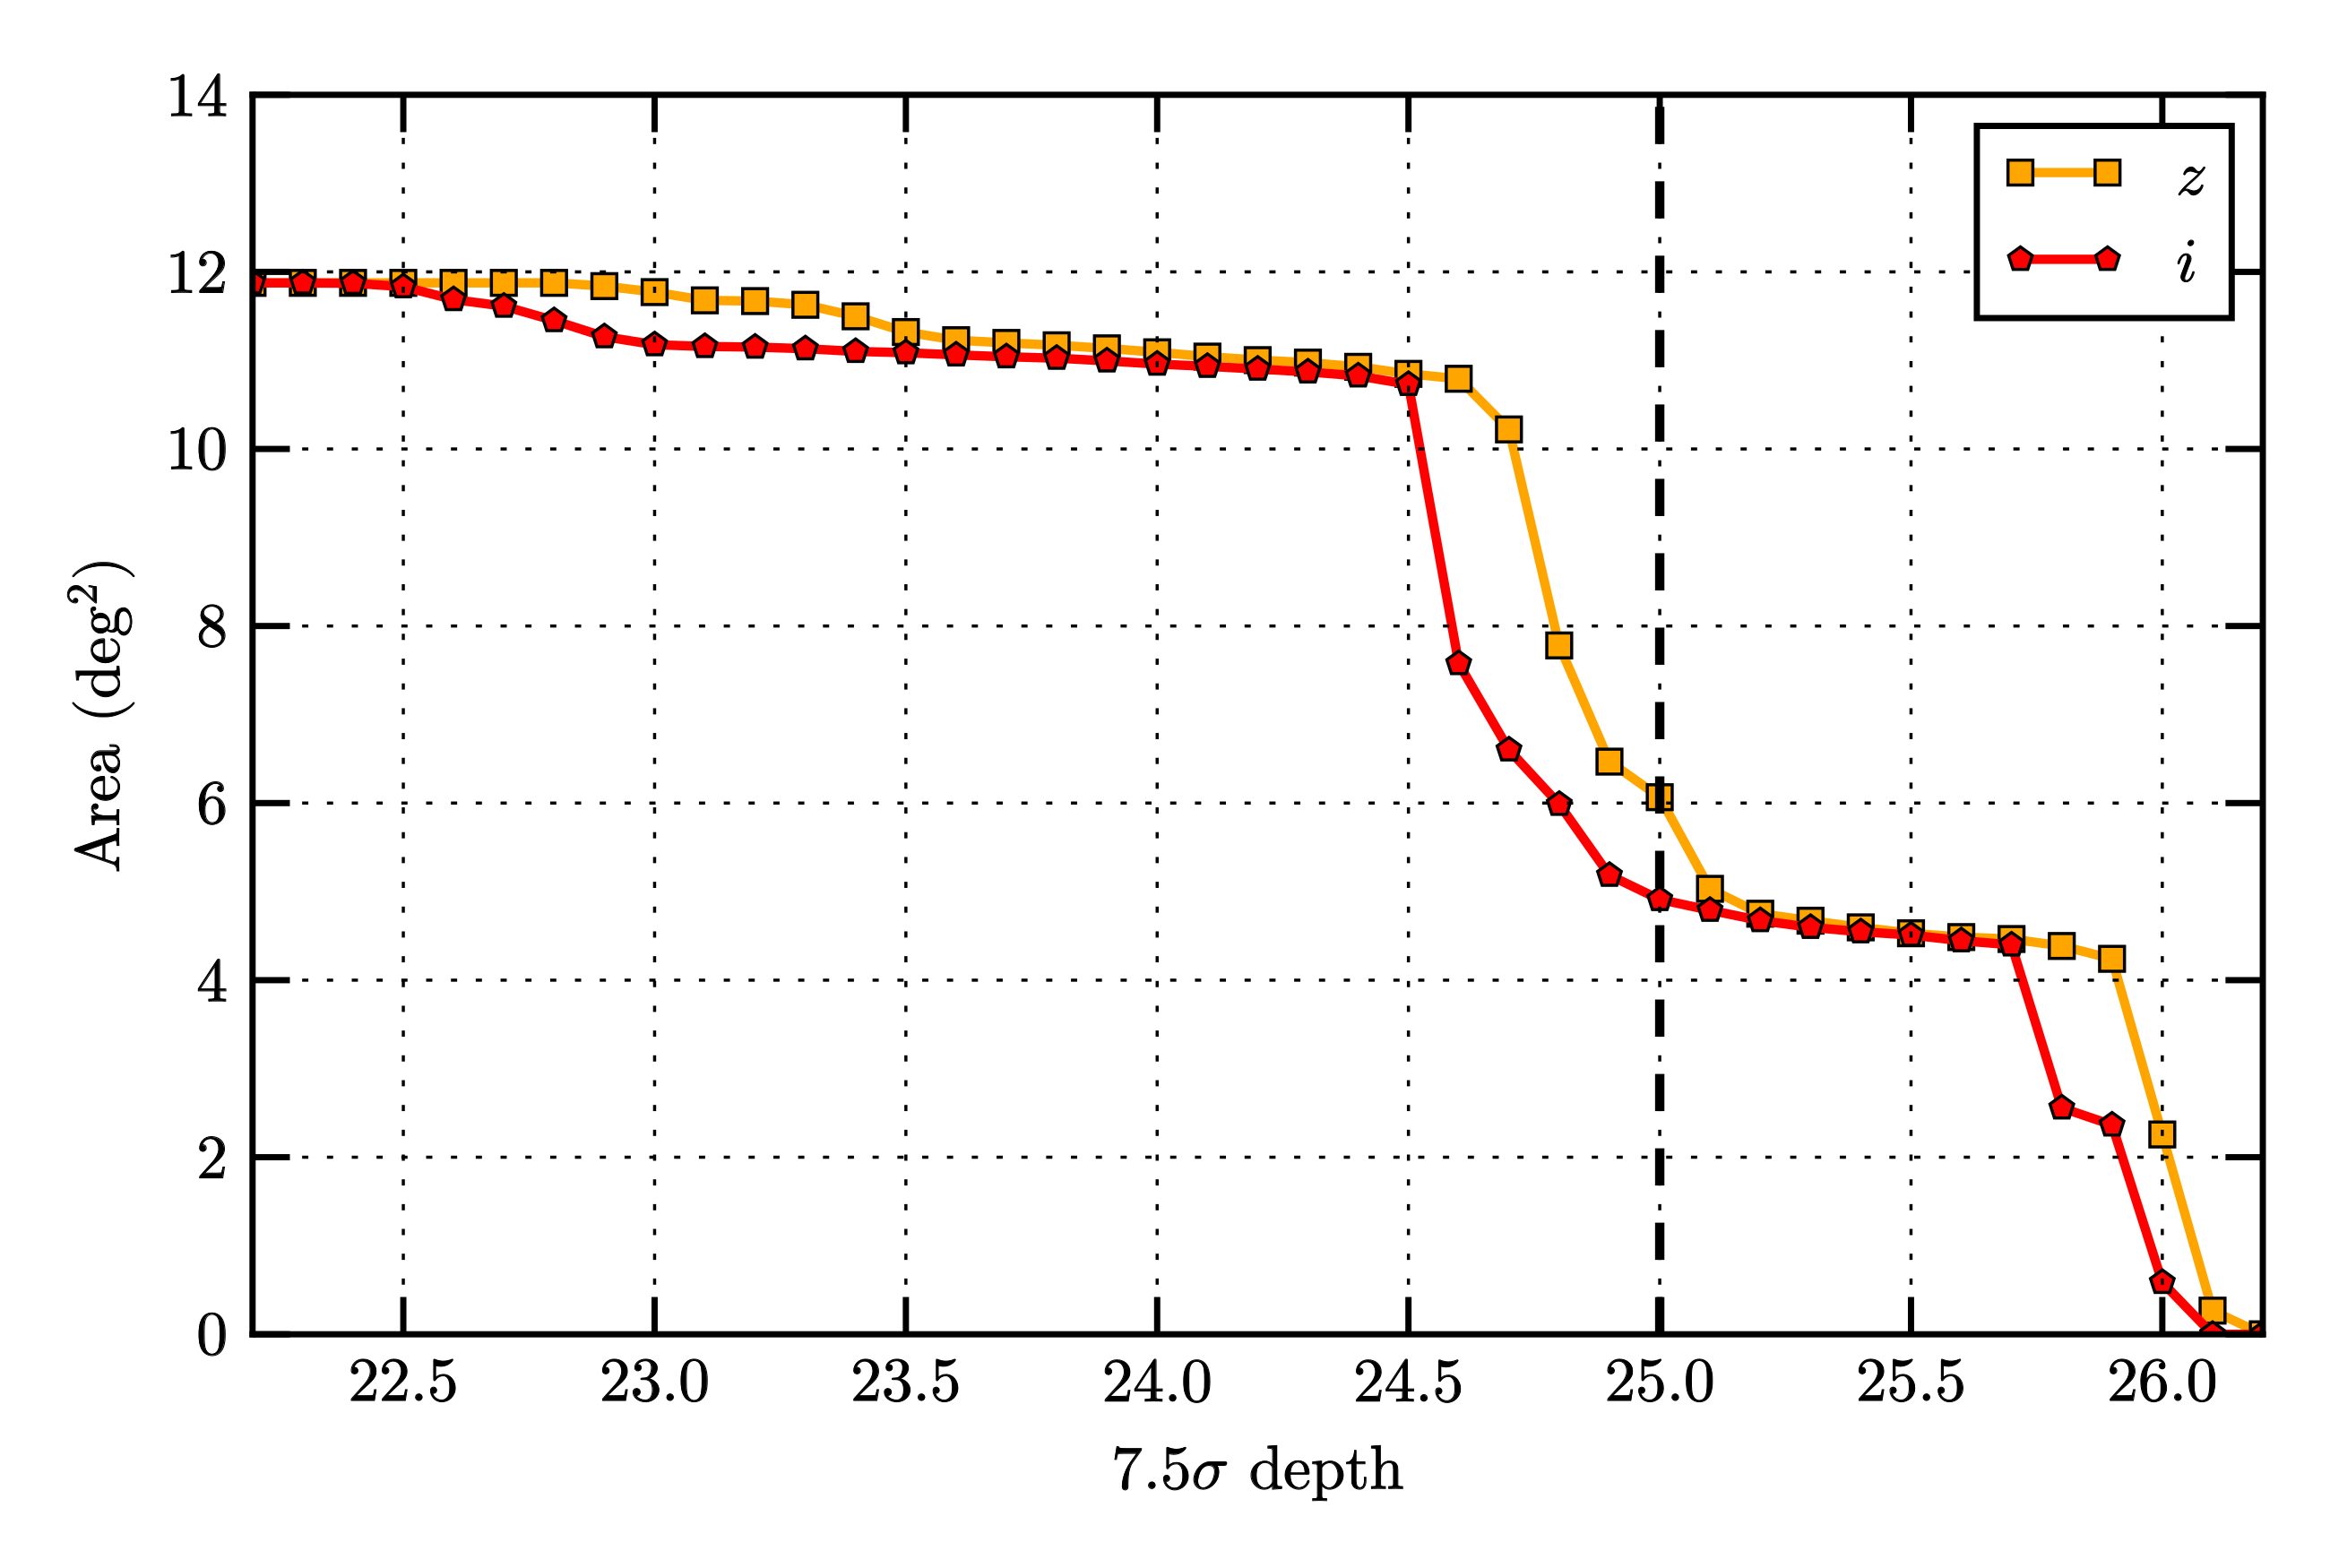
\includegraphics[width=0.95\textwidth]{Chapter4/Figs/area_depth_plot_7_5sig.png}
\caption[Area as a function of \texorpdfstring{$7.5\sigma$}{} depth for the \DESVIDEO footprint]{The area (with non-zero weight flags, see Section \ref{subsubsection:weight_flag_cut}) which is covered to a given $7.5\sigma$ depth as a function of that depth, for both the $i$-band and $z$-band data. The dashed vertical line signifies the $m_{\mathrm{AB}}< 25.0$ magnitude limit imposed in the candidate selection process.}
\label{fig:area_depth_7_5}
\end{figure}

For later reference, it is useful to point out that the DES $7.5\sigma$ depths are shallower than $m_{\mathrm{AB}} = 25.0$ in large regions of the \DESVIDEO footprint. Therefore, the magnitude/depth cut in Equation \ref{eqn:mag_cuts} has essentially restricted the high-redshift search to a smaller effective area --- i.e. the area with a $7.5\sigma$ limiting magnitude of $m_{7.5\sigma} > 25.0$. This is illustrated in Figure \ref{fig:area_depth_7_5}, which plots the available area to a given depth against depth (after excluding areas with bad weight flags defined in Section \ref{subsubsection:weight_flag_cut}). There is \SI{6.1}{\sqdeg} available to a $7.5\sigma$ limiting magnitude of $i_{\mathrm{AB}}< 25.0$, and \SI{4.9}{\sqdeg} to $z_{\mathrm{AB}}< 25.0$. \par 


\afterpage{
\clearpage
\begin{table}[p]
\centering
\begin{ThreePartTable}
%\setlength{\tabcolsep}{0.3em}
\textsc{Candidate Cuts} \\
\vspace{0.2em}
\begin{tabular}{lcclc}
\toprule
\multicolumn{2}{c}{\textsc{$z\sim5$ sample}} & & \multicolumn{2}{c}{\textsc{$z\sim6$ sample}}  \\
%\cmidrule{1-2} & & \cmidrule{4-5}\\
%\toprule\toprule
cut definition & remaining & \hspace{1.5em} & cut definition & remaining \\ 
\toprule\toprule 
\vspace{-0.8em}\\
Total catalogue\tnote{i} & \num{2443576} & & Total catalogue\tnote{i} & \num{2443576} \\ \midrule

\texttt{FLAGS\_WEIGHT}\tnote{ii} = 0 & \num{2375871} & & \texttt{FLAGS\_WEIGHT}\tnote{ii} = 0 & \num{2375871} \\[0.2em] \midrule

$4.83\leq z< 5.5$ & \num{14479} & & $5.5 \leq z< 6.5$ & 9899 \\[0.2em] \midrule

$\chi^2_{\nu,\mathrm{gal}} - \chi^2_{\nu,\mathrm{star}} <  -1.5$ & 572 & & $\chi^2_{\nu,\mathrm{gal}} - \chi^2_{\nu,\mathrm{star}} <  -1.5$ & 3504  \\[0.2em] \midrule

$\chi^2_{\nu,\mathrm{gal}}< 10$ & 386 & &  $\chi^2_{\nu,\mathrm{gal}}< 10$ & 1011 \\[0.2em] \midrule

\begin{tabular}{@{}l@{}}$i_{\mathrm{AB}}< 25.0$ \land \\ \hspace{0.2em} $\sigma_{i}< 0.1447$ ($7.5\sigma$)  \end{tabular} & 119 & & \begin{tabular}{@{}l@{}}$z_{\mathrm{AB}}< 25.0$ \land \\ \hspace{0.2em} $\sigma_{z}< 0.1447$ ($7.5\sigma$) \end{tabular} &  316 \\

\bottomrule
\end{tabular}
\vspace{0.2em}
\begin{tablenotes}
%\singlespacing
\setstretch{0.9}\small
\item[i] This catalogue consists of all sources in the \DESVIDEO footprint, including duplicates from overlapping DES or VIDEO tiles.
\item[ii] The requirement on \texttt{FLAGS\_WEIGHT} was imposed in all (observed) filters, so that `\texttt{FLAGS\_WEIGHT} = 0' is short for `$\texttt{FLAGS\_WEIGHT\_G} = 0 \land \texttt{FLAGS\_WEIGHT\_R} = 0 \land \texttt{FLAGS\_WEIGHT\_I} = 0 \land \texttt{FLAGS\_WEIGHT\_Z} = 0 \land \texttt{FLAGS\_WEIGHT\_Y} = 0 \land \texttt{FLAGS\_WEIGHT\_Z2} = 0 \land \texttt{FLAGS\_WEIGHT\_Y2} = 0 \land \texttt{FLAGS\_WEIGHT\_J} = 0 \land \texttt{FLAGS\_WEIGHT\_H} = 0 \land \texttt{FLAGS\_WEIGHT\_K} = 0$', where \texttt{Z} and \texttt{Y} refer to the DES $z$-band and $Y$-band, and \texttt{Z2} and \texttt{Y2} refer to the VIDEO $Z$-band and $Y$-band. 
\end{tablenotes}
\vspace{1em}
\caption[Selection criteria for the first round of cuts]{An overview of the selection criteria that have been applied to the total \DESVIDEO catalogue to obtain a preliminary sample of high-redshift candidate galaxies for visual inspection and further selection.}\label{table:preliminary_cuts}
\end{ThreePartTable}
\end{table}
\clearpage
}


\subsubsection{Conclusion of first round cuts}\label{subsubsection:first_cuts_summary}
The magnitude cuts above concluded the first selection round for the high-redshift search. Table \ref{table:preliminary_cuts} summarises all five selection criteria from this stage. Together, these broad initial cuts have generated a preliminary sample of 119 $z\sim5$ and 319 $z\sim6$ candidates,  to be narrowed down further by visual inspection and a second round of cuts described in the following sections. \par 

The observant reader may have noticed that the number of $z\sim6$ candidates in the preliminary sample is significantly higher than the number of $z\sim5$ candidates, which conflicts with the known behaviour of cosmic structure formation (as reflected, for instance, in the luminosity functions in Figure \ref{fig:luminosity_functions}, which show that the abundance of bright galaxies increases with decreasing redshift). This number disparity is partly caused by the fact that the $z\sim6$ sample includes a slightly wider redshift range than the $z\sim5$ sample. However, it was found during visual inspection that the main cause of the number difference is contamination by transients and artefacts in the $z\sim6$ sample. This issue will be addressed further in Section \ref{subsubsection:contamination_transients}. \par



\subsection{Visual inspection}\label{subsection:visual_inspection}
The next step in the selection process visually inspected each preliminary candidate. The aim of this stage, which is the topic of the current section, is to isolate any remaining contaminants. For this purpose, the author created a custom piece of code to produce an inspection image for each candidate object. Figure \ref{fig:example_transient} shows an example of such an image. \par 

Each inspection image consists of two parts. The top half is based on code written by Sophie Reed, and shows an array of fourteen \SI{30}{\arcsec} by \SI{30}{\arcsec} postage stamp cutouts of the object in various types of imaging. Nine of these cutouts show the nine \DESVIDEO bands used for computing photo-zs ($grizZYJHK_{s}$), with images left blank in bands where no data exists. The cutouts array also displays the DES $r+i+z$ detection image, as well as two false-colour images constructed from $g+r+i$ and $r+i+z$ images. The final two slots in the postage stamp array are filled with mid-infrared imaging from the \textit{Spitzer} Extragalactic Representative Volume Survey (SERVS; \citealt{2012PASP..124..714M}) in the IRAC CH1 (3.6$\mu$m) and CH2 (4.5$\mu$m) wavebands. This survey was conducted by the \textit{\textit{Spitzer}} Space Telescope in its post-cryogenic phase and covers an area of \SI{18}{\sqdeg} largely overlapping the \DESVIDEO footprint. With depths around $m_{\mathrm{AB}}\sim 23.1$ and a PSF FWHM of \SI{2}{\arcsec}, its image quality is considerably poorer than \DESVIDEO. Because of this, the SERVS data has not been used for the catalogue and photometric redshifts in this thesis. Evidence that the inclusion of IRAC fluxes does not improve photo-zs for many codes (around half of codes tested by \citealt{2010A&A...523A..31H}, including \texttt{LePHARE}) contributed to this decision. However, since the raw imaging does contain information that reflects the amount and extent of mid-IR emission, SERVS cutouts were considered valuable for the purpose of visual inspection. \par 


The second half of the inspection image consists of an SED plot that illustrates the photo-z fitting results for the candidate object in question. Measured magnitudes and magnitude errors are plotted in black for every (observed) filter, with the best-fit galaxy, star, and QSO templates overlaid in blue, yellow, and green respectively. For some candidates, \texttt{LePHARE} also found a secondary solution. As explained in Section \ref{subsubsection:chi_minimisation}, this occurs if the probability of the second-best galaxy redshift is above a certain user-specified threshold (chosen to be 0.1 in this thesis). If such a solution exists, it is overlaid in red. Magenta arrows show the $3\sigma$ depths in the area around the candidate object, as computed from Equations \ref{eqn:m_n} and \ref{eqn:m_n_video} (the top of the arrow corresponds to the $3\sigma$ depth). Inside the SED plot, a smaller inlay shows the probability distribution $P(z)$ as a function of redshift, computed by \texttt{LePHARE} during photometric redshift fitting (see Equation \ref{eqn:prob_func}). \par

Together, the combination of postage stamp images and SEDs contains a wealth of photometric and morphological clues. This information was then used to identify possible contaminants in the preliminary sample. The process unveiled several major types of contamination, which will be discussed below. \par 




\subsubsection{Contamination from transient emission and imaging artefacts}\label{subsubsection:contamination_transients}

\begin{figure}[tb]
\centering
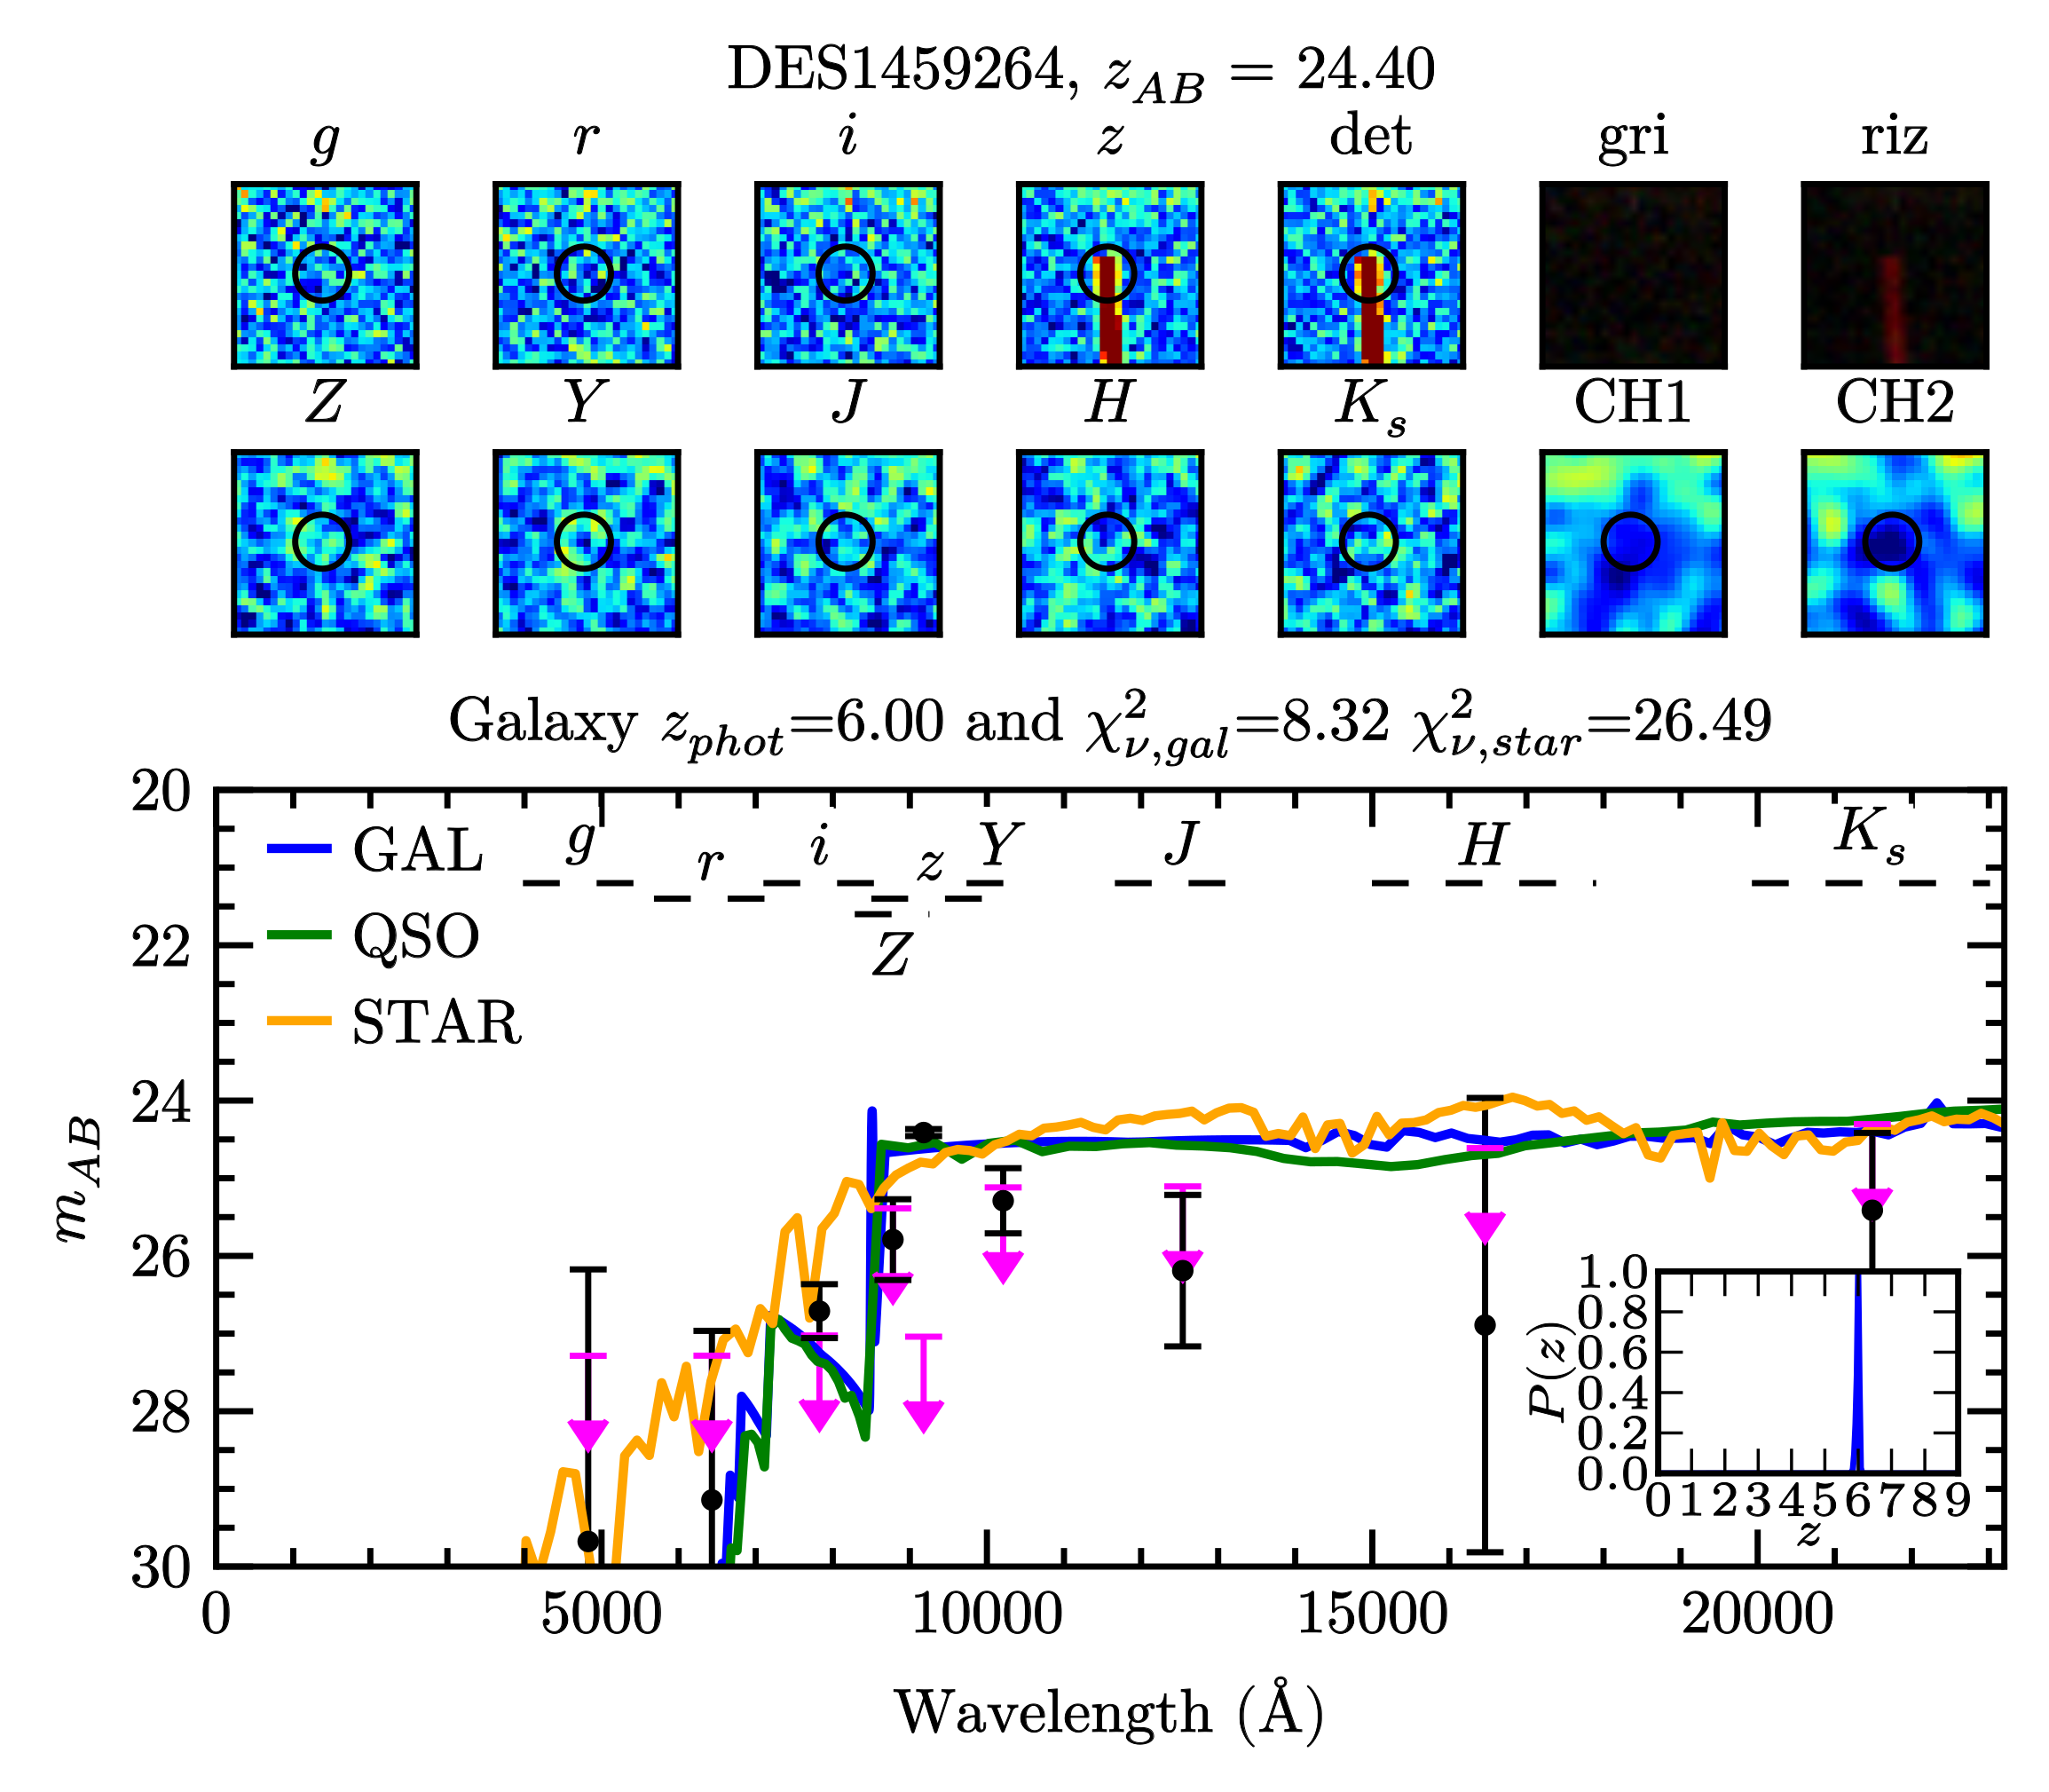
\includegraphics[width=0.95\textwidth]{Chapter4/Figs/DES1459264_thesis.png}
\caption[Example of contamination from a transient]{Verification image showing an example of contamination from a moving object. As the object happened to be in the field-of-view while a $z$-band exposure was taken, it only appears in that filter, mimicking a Lyman break between $i$ and $z$. On top of that, the errors in the redder (VIDEO) filters are large enough that the random background flux is compatible with galaxy continuum emission so that its best galaxy fit passed the required $\chi_{\nu,\mathrm{gal}}<10.0$ preliminary cut.}
\label{fig:example_transient}
\end{figure}

The most easily distinguishable type of contamination consists of objects that are neither stars nor galaxies of any sort. Specifically, this category is comprised of imaging artefacts and transient emission. The latter kind was found to occur the most often, due to cosmic rays as well as moving extended sources such as asteroids, airplanes, or satellites. Transients were easily identified in the postage stamp cutouts via two main distinguishing properties. Firstly, the shape of the emission provided crucial evidence: spikes from fast-moving objects show up as bright elongated trails, and slower asteroids or satellites often look like resolved spheroids that are bright all over (as opposed to galaxies or stars whose light profiles look like ellipsoids, disks, or PSFs). Secondly, transients only show up in one filter, because they temporarily appeared in the field-of-view while that waveband was being exposed. The reason why such time-variable objects can infiltrate the preliminary sample is to do with this second property. If a bright transient happens to appear in the detection band, its observed SED can mimic the spectrum of high-redshift Lyman-break galaxies.  This is because the lack of flux bluewards of the detection band can replicate the characteristic LBG dropout behaviour shortwards of the Lyman break, while the strong emission in the detection band can imitate the expected strong continuum flux in the rest-frame UV. In some of these cases, the  photometry redwards of the detection band is consistent with LBG continuum emission, for instance if the data contains sufficiently large photometric errors in these redder bands, or if the contaminant overlaps with a real object, a random spike in background emission, or an artefact (see below). \texttt{LePHARE} may assign such transients a high-redshift solution, which, if the errors in the redder bands are large enough, can have a $\chi^2_{\nu,\mathrm{gal}}$ within the range from the preliminary cuts. An example of a transient contaminant is shown in Figure \ref{fig:example_transient}. \par 

\begin{figure}[tb]
\centering
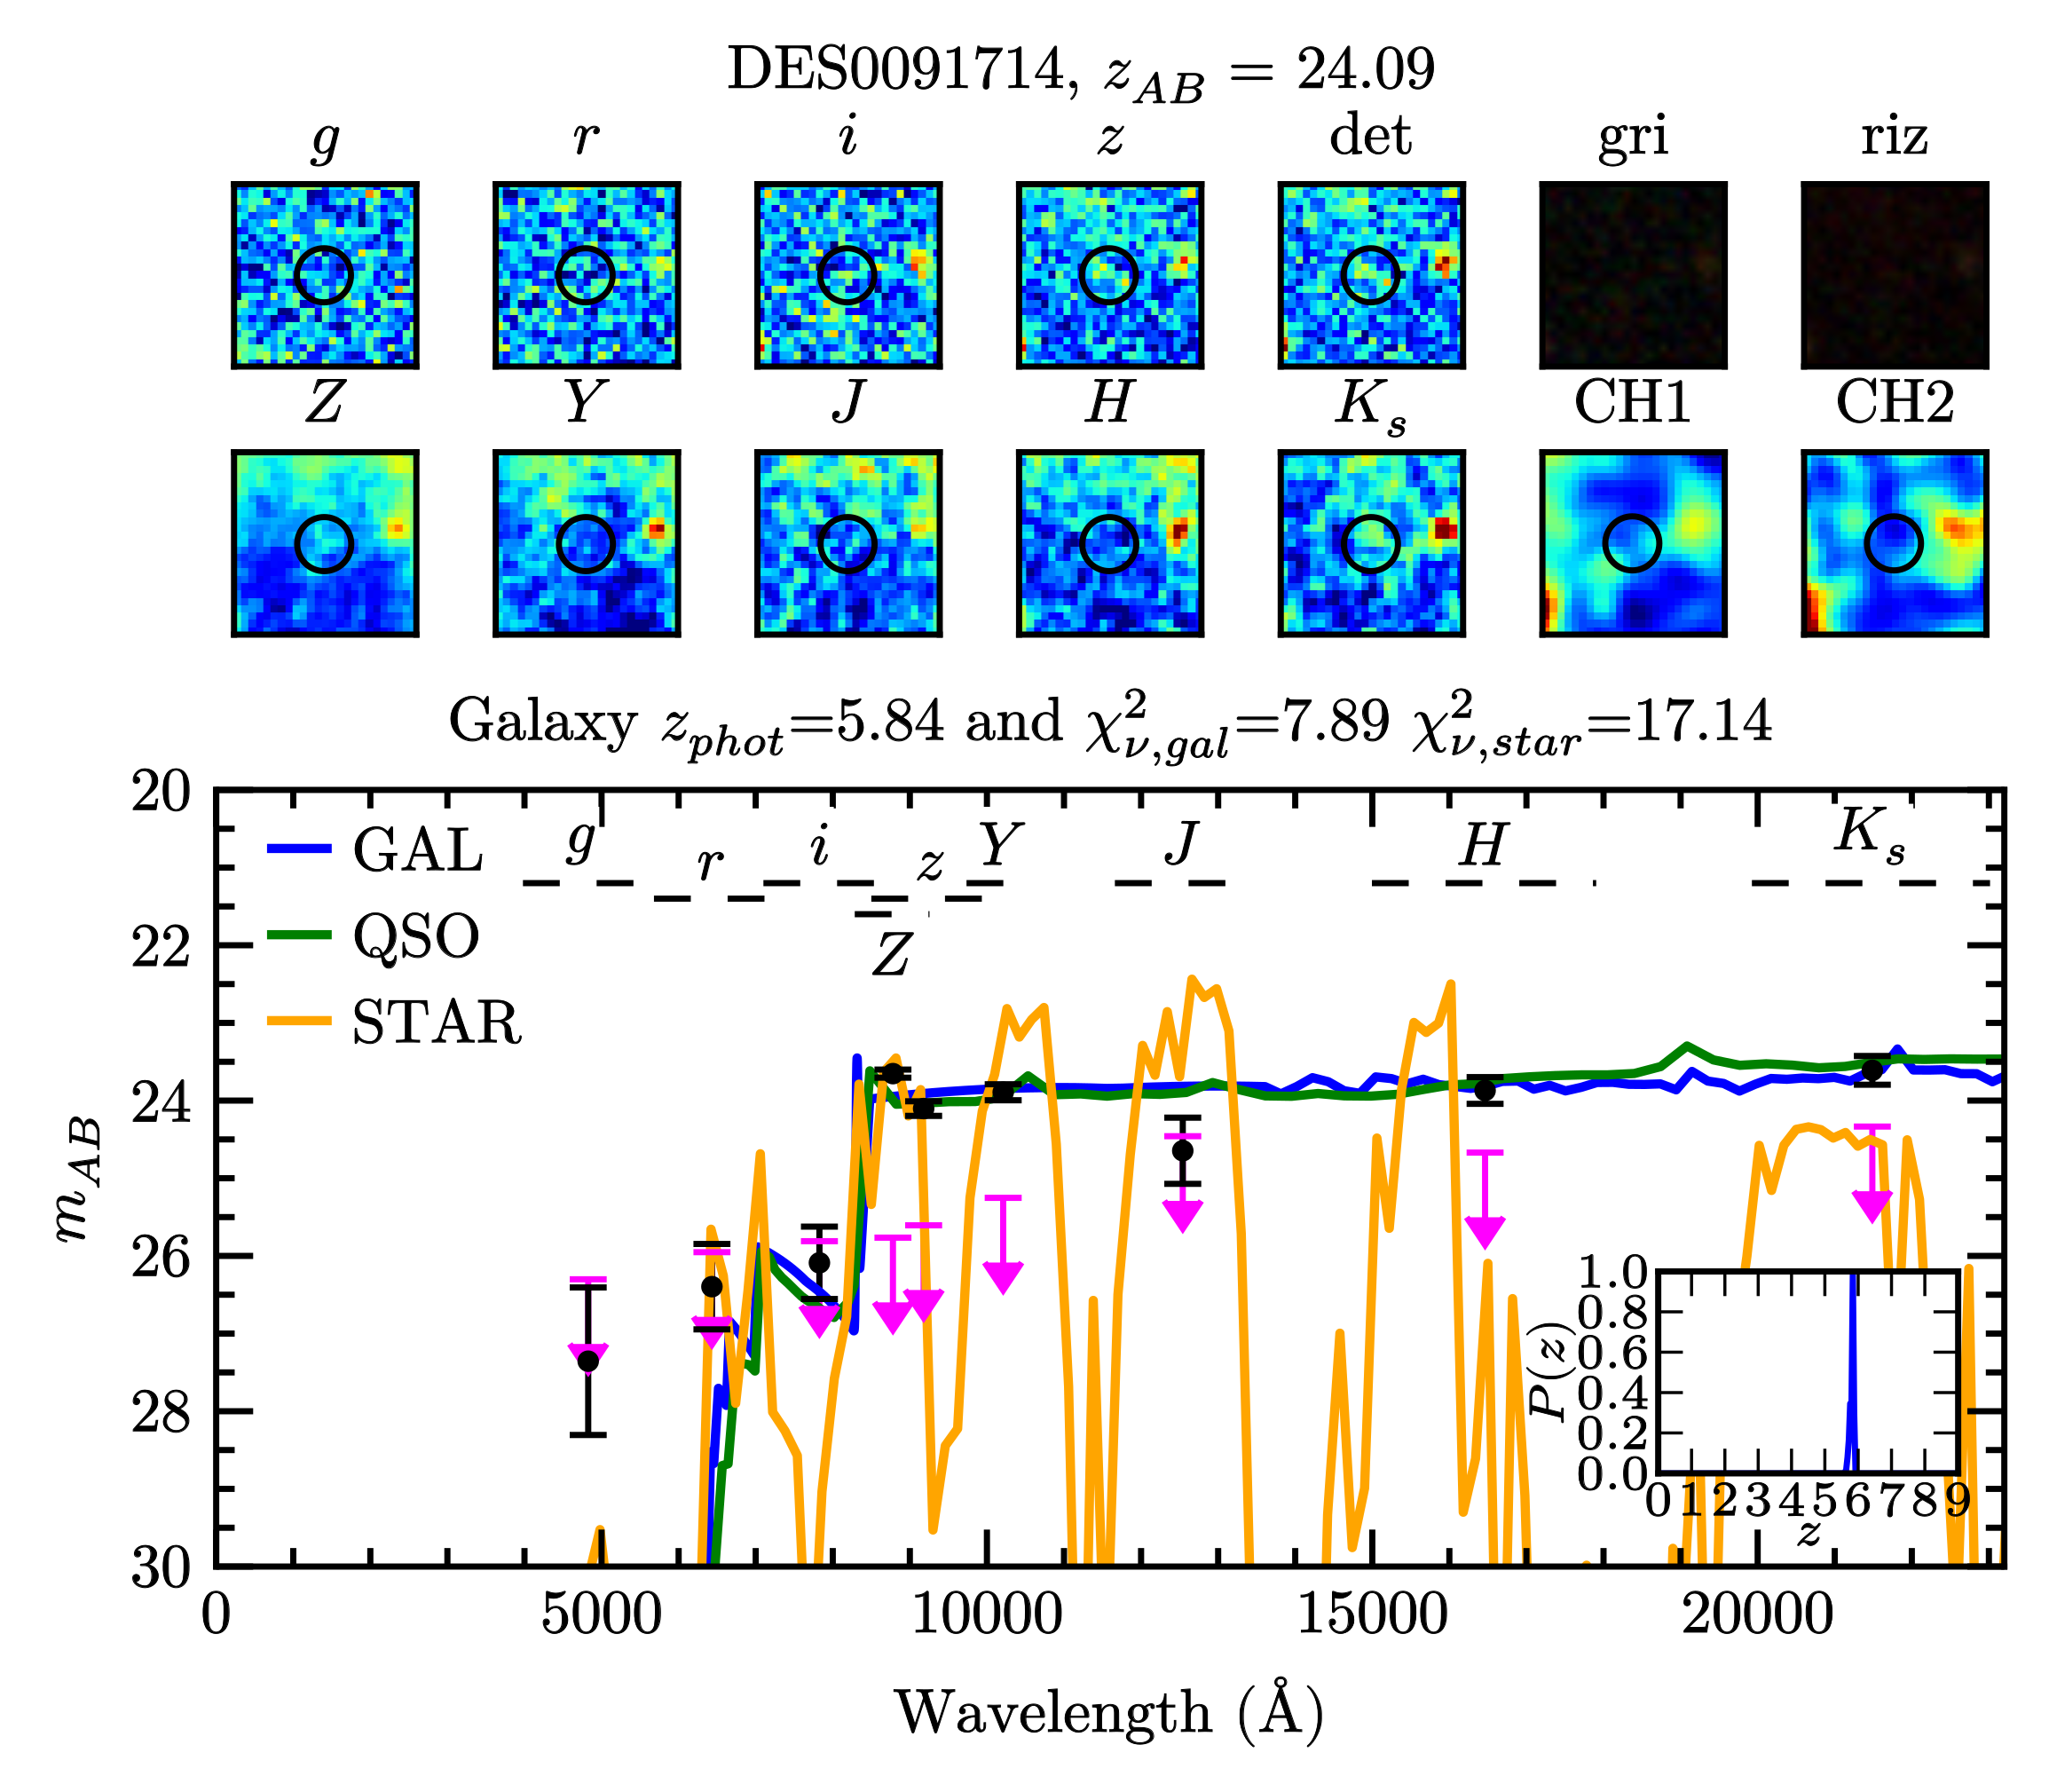
\includegraphics[width=0.95\textwidth]{Chapter4/Figs/DES0091714_thesis.png}
\caption[Example of contamination from an imaging artefact]{An example of contamination caused by imaging artefacts. Zooming out on the imaging for this contaminant revealed that the diffuse background emission in the postage stamps is caused by the extended PSF of a very bright nearby star. The random $z$-band spike in this PSF flux turns out to be bright enough to pass the \texttt{SExtractor} detection threshold, so that it shows up as a phantom detection in the \DESVIDEO catalogue. Because the nearby star is particularly luminous in the near-IR, its colours fairly closely replicate those of true high-redshift galaxies, which caused this phantom detection to make it into the preliminary sample.}
\label{fig:example_artefact}
\end{figure}

Imaging artefacts form another category of contaminant that was identified during visual inspection. Since imaging faults do not represent any external light source at all, these sorts of objects are `phantom' detections. The most common type of artefact contamination was found to be extended emission in the PSF of very bright stars (including diffraction spikes). Occasionally, random fluctuations in this stellar emission are bright enough to pass the object detection threshold in \texttt{SExtractor}, causing them to appear as phantom objects in the \DESVIDEO catalogue. In some cases, their colours are sufficiently like true high-redshift galaxies that these sources entered the preliminary sample. Figure \ref{fig:example_artefact} shows an example of contamination from the extended PSF of a bright star. \par


%In addition to moving objects and cosmic rays, imaging artefacts form a third category of junk contaminant.


Contamination from transients and artefacts was found exclusively in the $z\sim6$ sample. This is the primary cause of the discrepancy between the number of $z\sim5$ and $z\sim6$ preliminary candidates noted previously in Section \ref{subsubsection:first_cuts_summary}. The discussion will now turn to why this contamination specifically occurs at $z\sim6$. Two main reasons can be identified. Firstly, the DES data is generally deeper than VIDEO, so the VIDEO photometric uncertainties are typically larger than those in DES. On top of that, near-infrared imaging also suffers from higher atmospheric background noise, which can lead to random bright spots within the VIDEO data, especially if the background subtraction was not performed perfectly. As a result, compared to DES, the VIDEO photometry is more likely to be consistent with the expected continuum emission from a high-redshift galaxy, even if there is no real object present. At $z\sim6$, all imaging redwards of the detection band lies within VIDEO, so a $z$-band transient can mimic a true $z\sim6$ LBG due to this lower VIDEO data quality. On the other hand, any $i$-band transient would also need to show bright continuum emission in the DES $z$-band to be compatible with a $z\sim5$ LBG, which is less likely thanks to the higher DES image quality. The second reason why contamination from transients and artefacts is less probable among $z\sim5$ candidates, is that a $z\sim5$ candidate requires continuum emission to be detected in one additional filter compared to $z\sim6$ objects (i.e. $izZYJHK_{s}$ instead of $zZYJHK_{s}$). If the object is not a true high-redshift LBG, the inconsistency between the measured contaminant flux and the high-redshift template flux in this additional filter will increase its $\chi^2_{\nu,\mathrm{gal}}$, which significantly decreases the chances of this object making it into the preliminary candidate sample. \par


\subsubsection{Contamination from low-redshift galaxies and QSOs}\label{subsubsection:contamination_low_z}
Visual inspection also uncovered low-redshift galaxies as another major type of contaminant. While these were not always quite as straightforward to identify as the earlier `junk' objects, the inspection images nevertheless contain various key indicators. These distinguishing characteristics will be described below.  \par

The first way to identify low-redshift contamination is via flux bluewards of the Lyman break. As explained in Section \ref{subsubsection:lyman_break}, true Lyman-break galaxies show virtually no emission shortwards of \SI{912}{\angstrom}, and a strong (redshift dependent) lack of flux between \SI{912}{\angstrom} and \SI{1216}{\angstrom}. Objects which contain blue flux incompatible with these limits can therefore not be true high-redshift galaxies. In addition to low-redshift interlopers, blue light could theoretically also originate from stars. However, this is much less likely in a high-redshift sample, since the types of stars that are compatible with the colours of $z\gtrsim5$ galaxies are M, L, and T (brown) dwarfs, which are undetectable in blue filters. Regardless, even if it is stellar in origin, excess blue flux indicates contamination. For the $z\sim5$ sample, such an excess consists of any emission in the $g$-band, and any $r$-band flux that is brighter than the typical $r_{\mathrm{AB}}-i_{\mathrm{AB}}$ drop values of around 1 to 2 (or more) expected for $r$-dropouts based on observational studies \citep{2004AJ....127.2598S,2010A&A...523A..74V}. Similarly, contamination in the $z\sim6$ sample can be confirmed through the presence of $g$-band emission, a \SI{912}{\angstrom} drop in $r$-band flux smaller than the expected $r_{\mathrm{AB}}-z_{\mathrm{AB}}\gtrsim 3$ break (such a drop manifests as a non-detection in $r$ in almost all cases), or a \SI{1216}{\angstrom} drop less than the expected $i_{\mathrm{AB}}-z_{\mathrm{AB}}$ break of at least 2 or 3 (all the above colours have been derived from observations; \citealt{2004AJ....127.2598S,2015MNRAS.452.1817B,2013AJ....145....4W}). During visual inspection, these requirements exposed several preliminary candidates as contaminants,  either because they show $g$-band emission in the cutouts, or because their Lyman breaks are not strong enough in the SED plots. On top of that, a further set of preliminary candidates was marked as highly uncertain on the basis that their imaging is too noisy\footnote{These noisy regions lie mainly in the proximity of chip gaps.} in the designated blue filters to rule out an excess of blue flux. To ensure maximum purity of the final high-redshift sample, these dubious sources were also classified as contaminants. An example is shown in Figure \ref{fig:example_g_noise}. \par

\begin{figure}[tb]
\centering
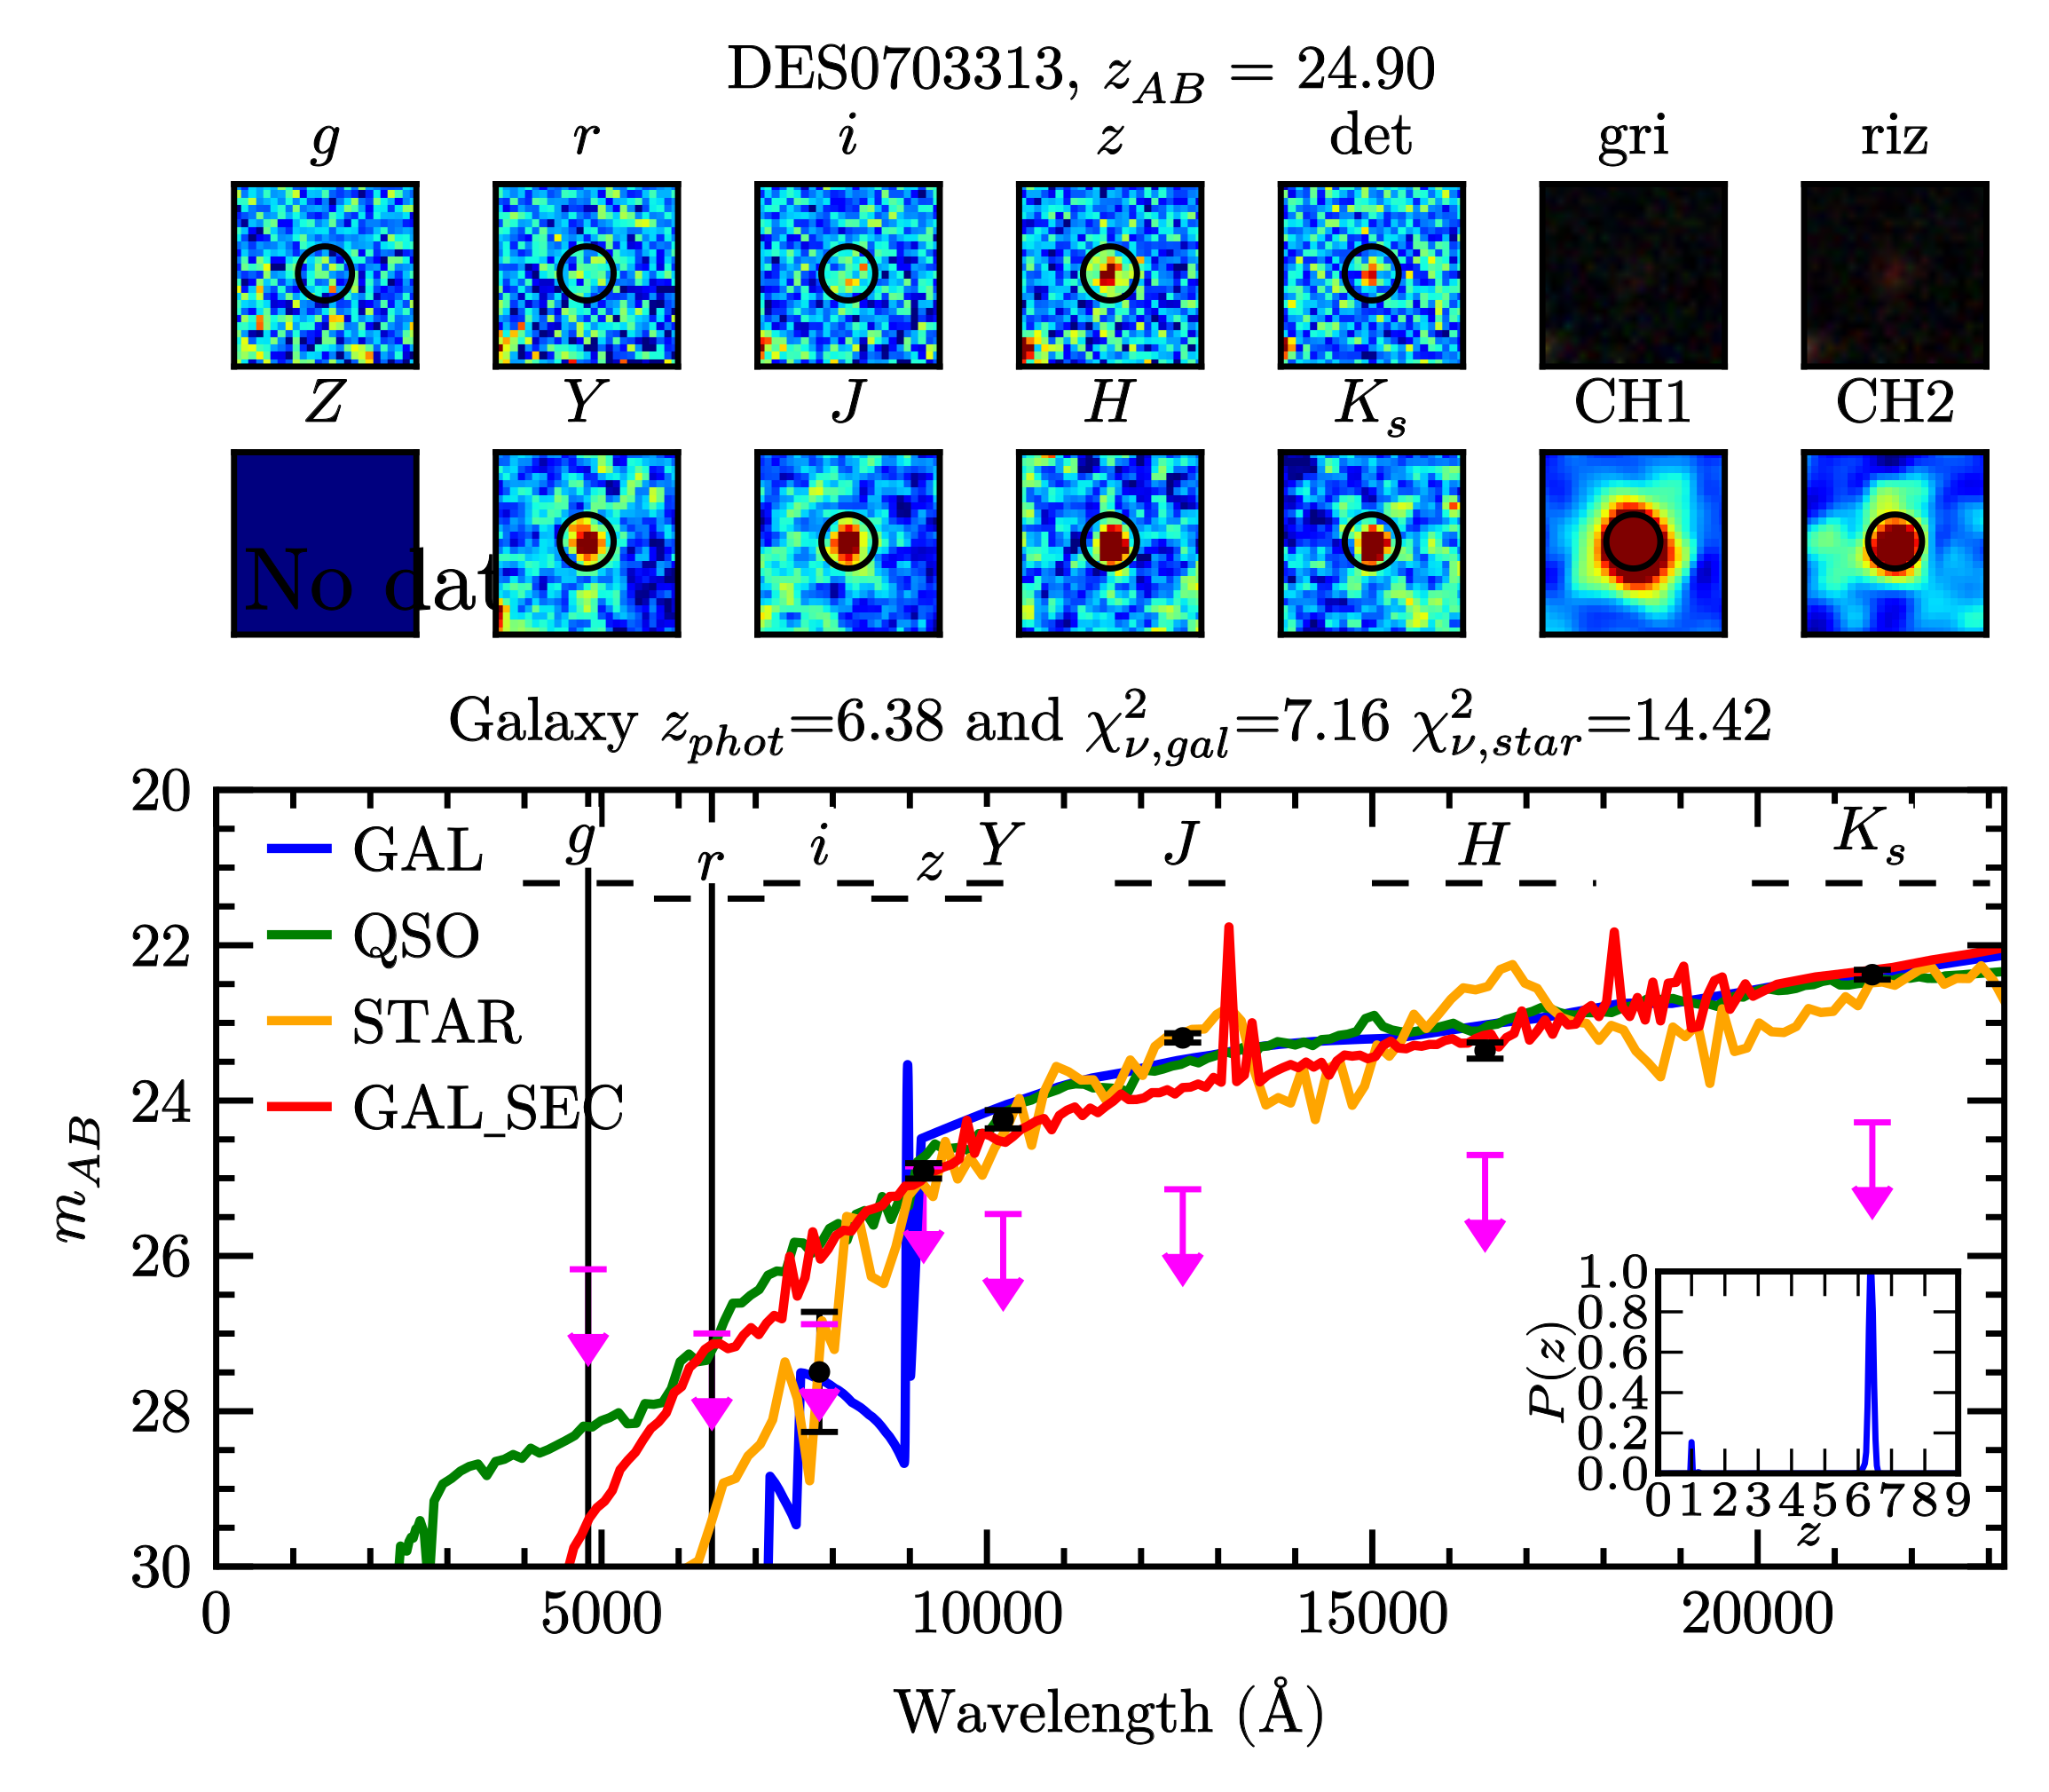
\includegraphics[width=0.95\textwidth]{Chapter4/Figs/DES0703313_thesis.png}
\caption[Example of low-redshift contamination due to \texorpdfstring{$g$}{}-band and \texorpdfstring{$r$}{}-band  noise]{An example of  low-redshift contamination likely caused by noisy photometry in the $g$- and $r$-band (due to close proximity to the chip gaps). On the whole, the object shows clear signs of a low-redshift origin, such as a gently sloping SED and bright \textit{Spitzer} emission. Due to the high noise in the $g$- and $r$-band imaging, the object did not pass the \texttt{SExtractor} detection threshold in these bands, mimicking the flux measurements of an $i$-dropout. However, visual examination of the $g$- and $r$-band cutouts suggests that these wavebands do contain some flux that was missed due to the high noise.}
%the object is removed as a potential quasar or secondary solution
\label{fig:example_g_noise}
\end{figure}


A second strategy to identify low-redshift contaminants looked at the shape of their observed SEDs. Since their photometry must be sufficiently similar to true high-redshift galaxies to have passed the first round of preliminary cuts, their intrinsic spectra need to be exceptionally red, implying that they must be extremely dusty. The SEDs of intrinsically red sources generally show a more gently sloping increase than typical Lyman-break galaxies, and their observed colours often continue getting redder into the near-infrared regime (whereas Lyman-break galaxies show blue colours longwards of the Lyman break). Because they are so dusty, they also often display bright mid-IR emission in the \textit{Spitzer} CH1 and CH2 cutouts. During visual inspection, several preliminary candidates were found to show such photometry indicative of a red low-redshift galaxy. It is suspected that this failure by \texttt{LePHARE} to correctly identify some very red galaxies may be due to inaccurate photometry, or template incompleteness at the extreme red end. Regarding the former issue, the inspection image SED plots of many low-redshift contaminants indeed sometimes indicate that $\chi^2_{\nu,\mathrm{gal}}$ might have been biased by one or two bands with very small errors, while the other bands look more compatible with a low-redshift fit. This hypothesis is supported by the fact that the best-fit solution for most (89\%) objects in the preliminary sample has a reduced chi-squared of $\chi_{\nu}^2>1$, which suggests that the photometric uncertainties in at least some bands may be slightly too small compared to the template set. For another class of low-redshift contaminants, it was found that the false high-redshift outcome has likely been biased by data in noisy regions (as previously seen in Figure \ref{fig:example_g_noise}) or nearby sources. Figure \ref{fig:example_low_z} presents an example of the latter cause. \par


\begin{figure}[tb]
\centering
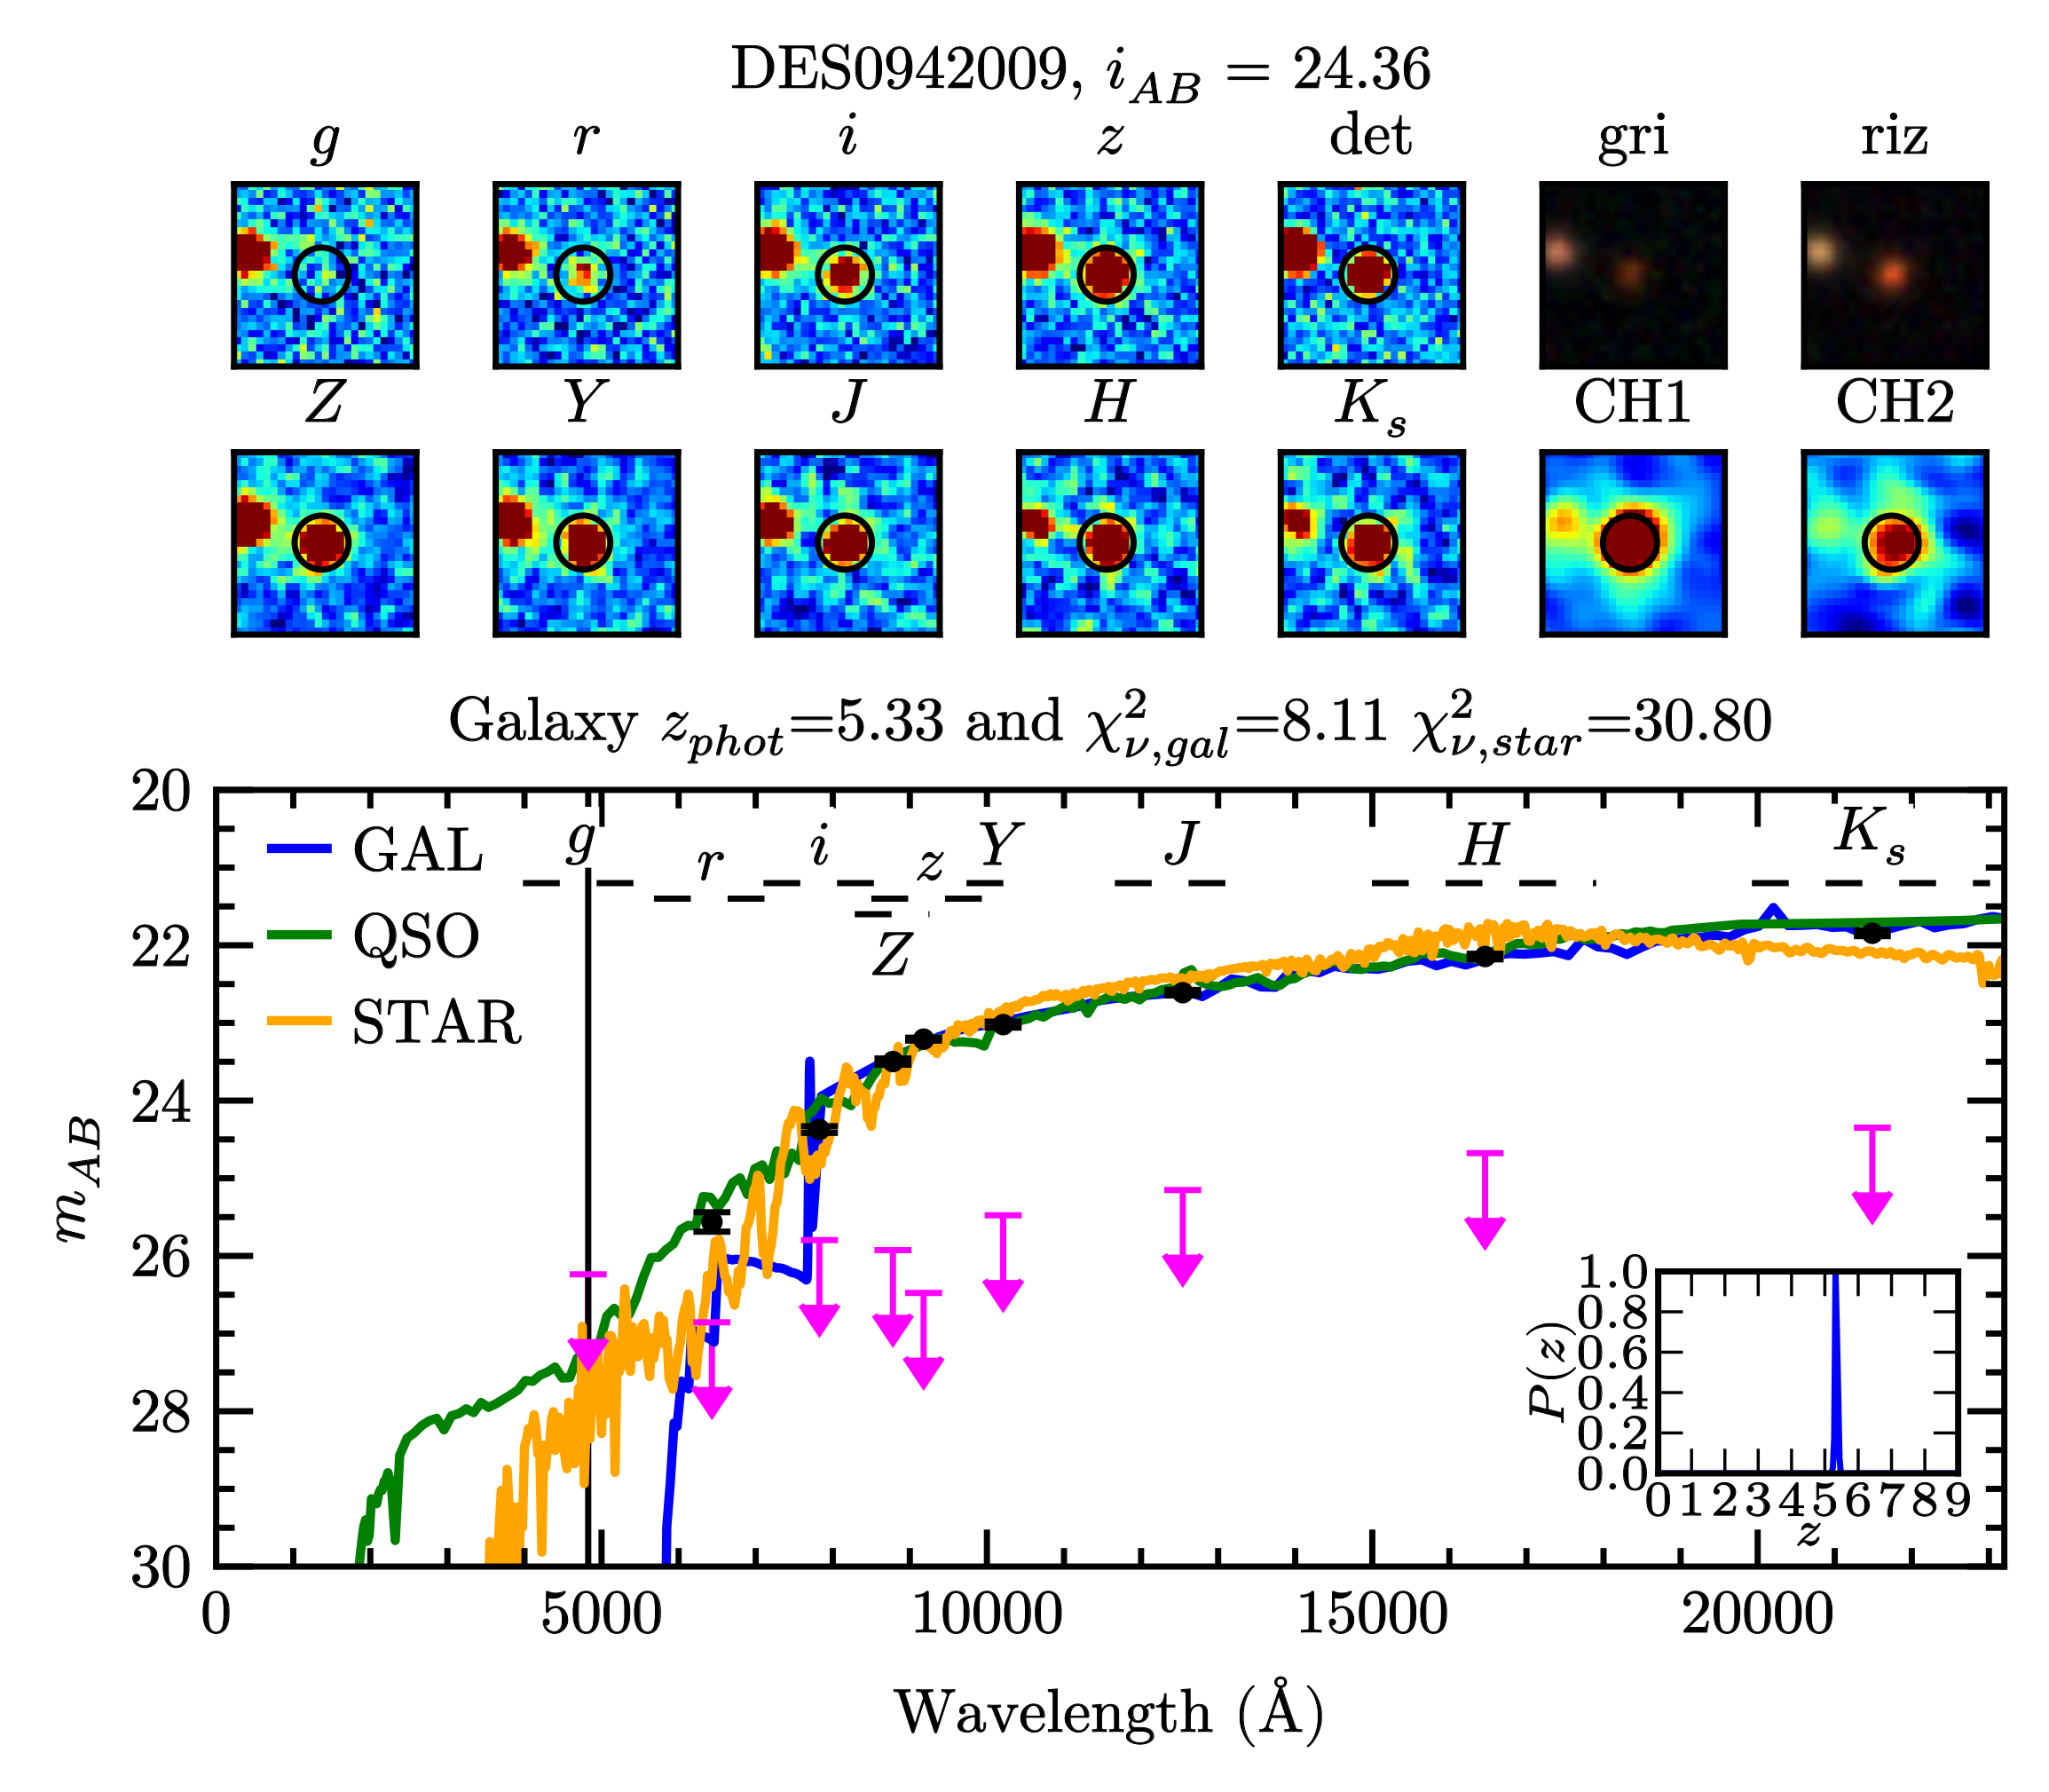
\includegraphics[width=0.95\textwidth]{Chapter4/Figs/DES0942009_thesis.png}
\caption[Example of a low-redshift contaminant]{An example of low-redshift contamination likely caused by flux from a nearby source to the left. Like the low-redshift interloper in Figure \ref{fig:example_g_noise}, this object shows a gently sloping SED (note the lack of a strong $r-i$ break) and luminous \texttt{Spitzer} emission, both indicating a low-redshift origin. It is likely that the galaxy fit was biased by very small errors in some bands where the flux was boosted by a bright neighbour. }
%sloping SED, QSO solution, flux affected by nearby object
\label{fig:example_low_z}
\end{figure}


Inbuilt features in \texttt{LePHARE} can provide further ways to distinguish potential low-redshift contaminants. One such strategy utilised secondary redshift solutions, which, if present\footnote{As explained in Sections \ref{subsubsection:chi_minimisation} and \ref{subsection:visual_inspection}, a secondary solution exists if the probability function $P(z)$ is larger than 0.1 at the second most probable photometric redshift.}, are plotted in the inspection images. Several preliminary candidates were found to have secondary redshifts between $0<z_{\mathrm{sec}}<2$, indicating that their photometry is compatible with a low-redshift origin. The contaminant previously introduced in Figure \ref{fig:example_g_noise} is an example of such an object with a secondary solution around $z_{\mathrm{sec}}\approx1$. Because it is important that all final candidates are maximally secure, any preliminary candidates with a low-redshift secondary solution were considered contaminants. \par 

%I GOT UP TO HERE

A further useful feature in \texttt{LePHARE} is the ability to fit QSO templates (see Section \ref{subsection:star_qso_templates}), which helped to identify preliminary candidates that could be low-redshift quasars. Since each inspection image contains the best-fit QSO template, potential low-redshift QSOs could easily be recognised in the SED plots. During visual inspection, it was found that several preliminary candidates have a reasonable quasar solution at low-redshift. In many cases, the photometry for these sources indeed shows signs of low-redshift emission, such as gently sloping SEDs similar to those of the low-redshift galaxies found earlier. Again, to ensure maximal purity, objects with a good low-redshift QSO fit were flagged as contaminants. \par 


\subsubsection{Contamination from stars}\label{subsubsection:contamination_stars}

\begin{figure}[tb]
\centering
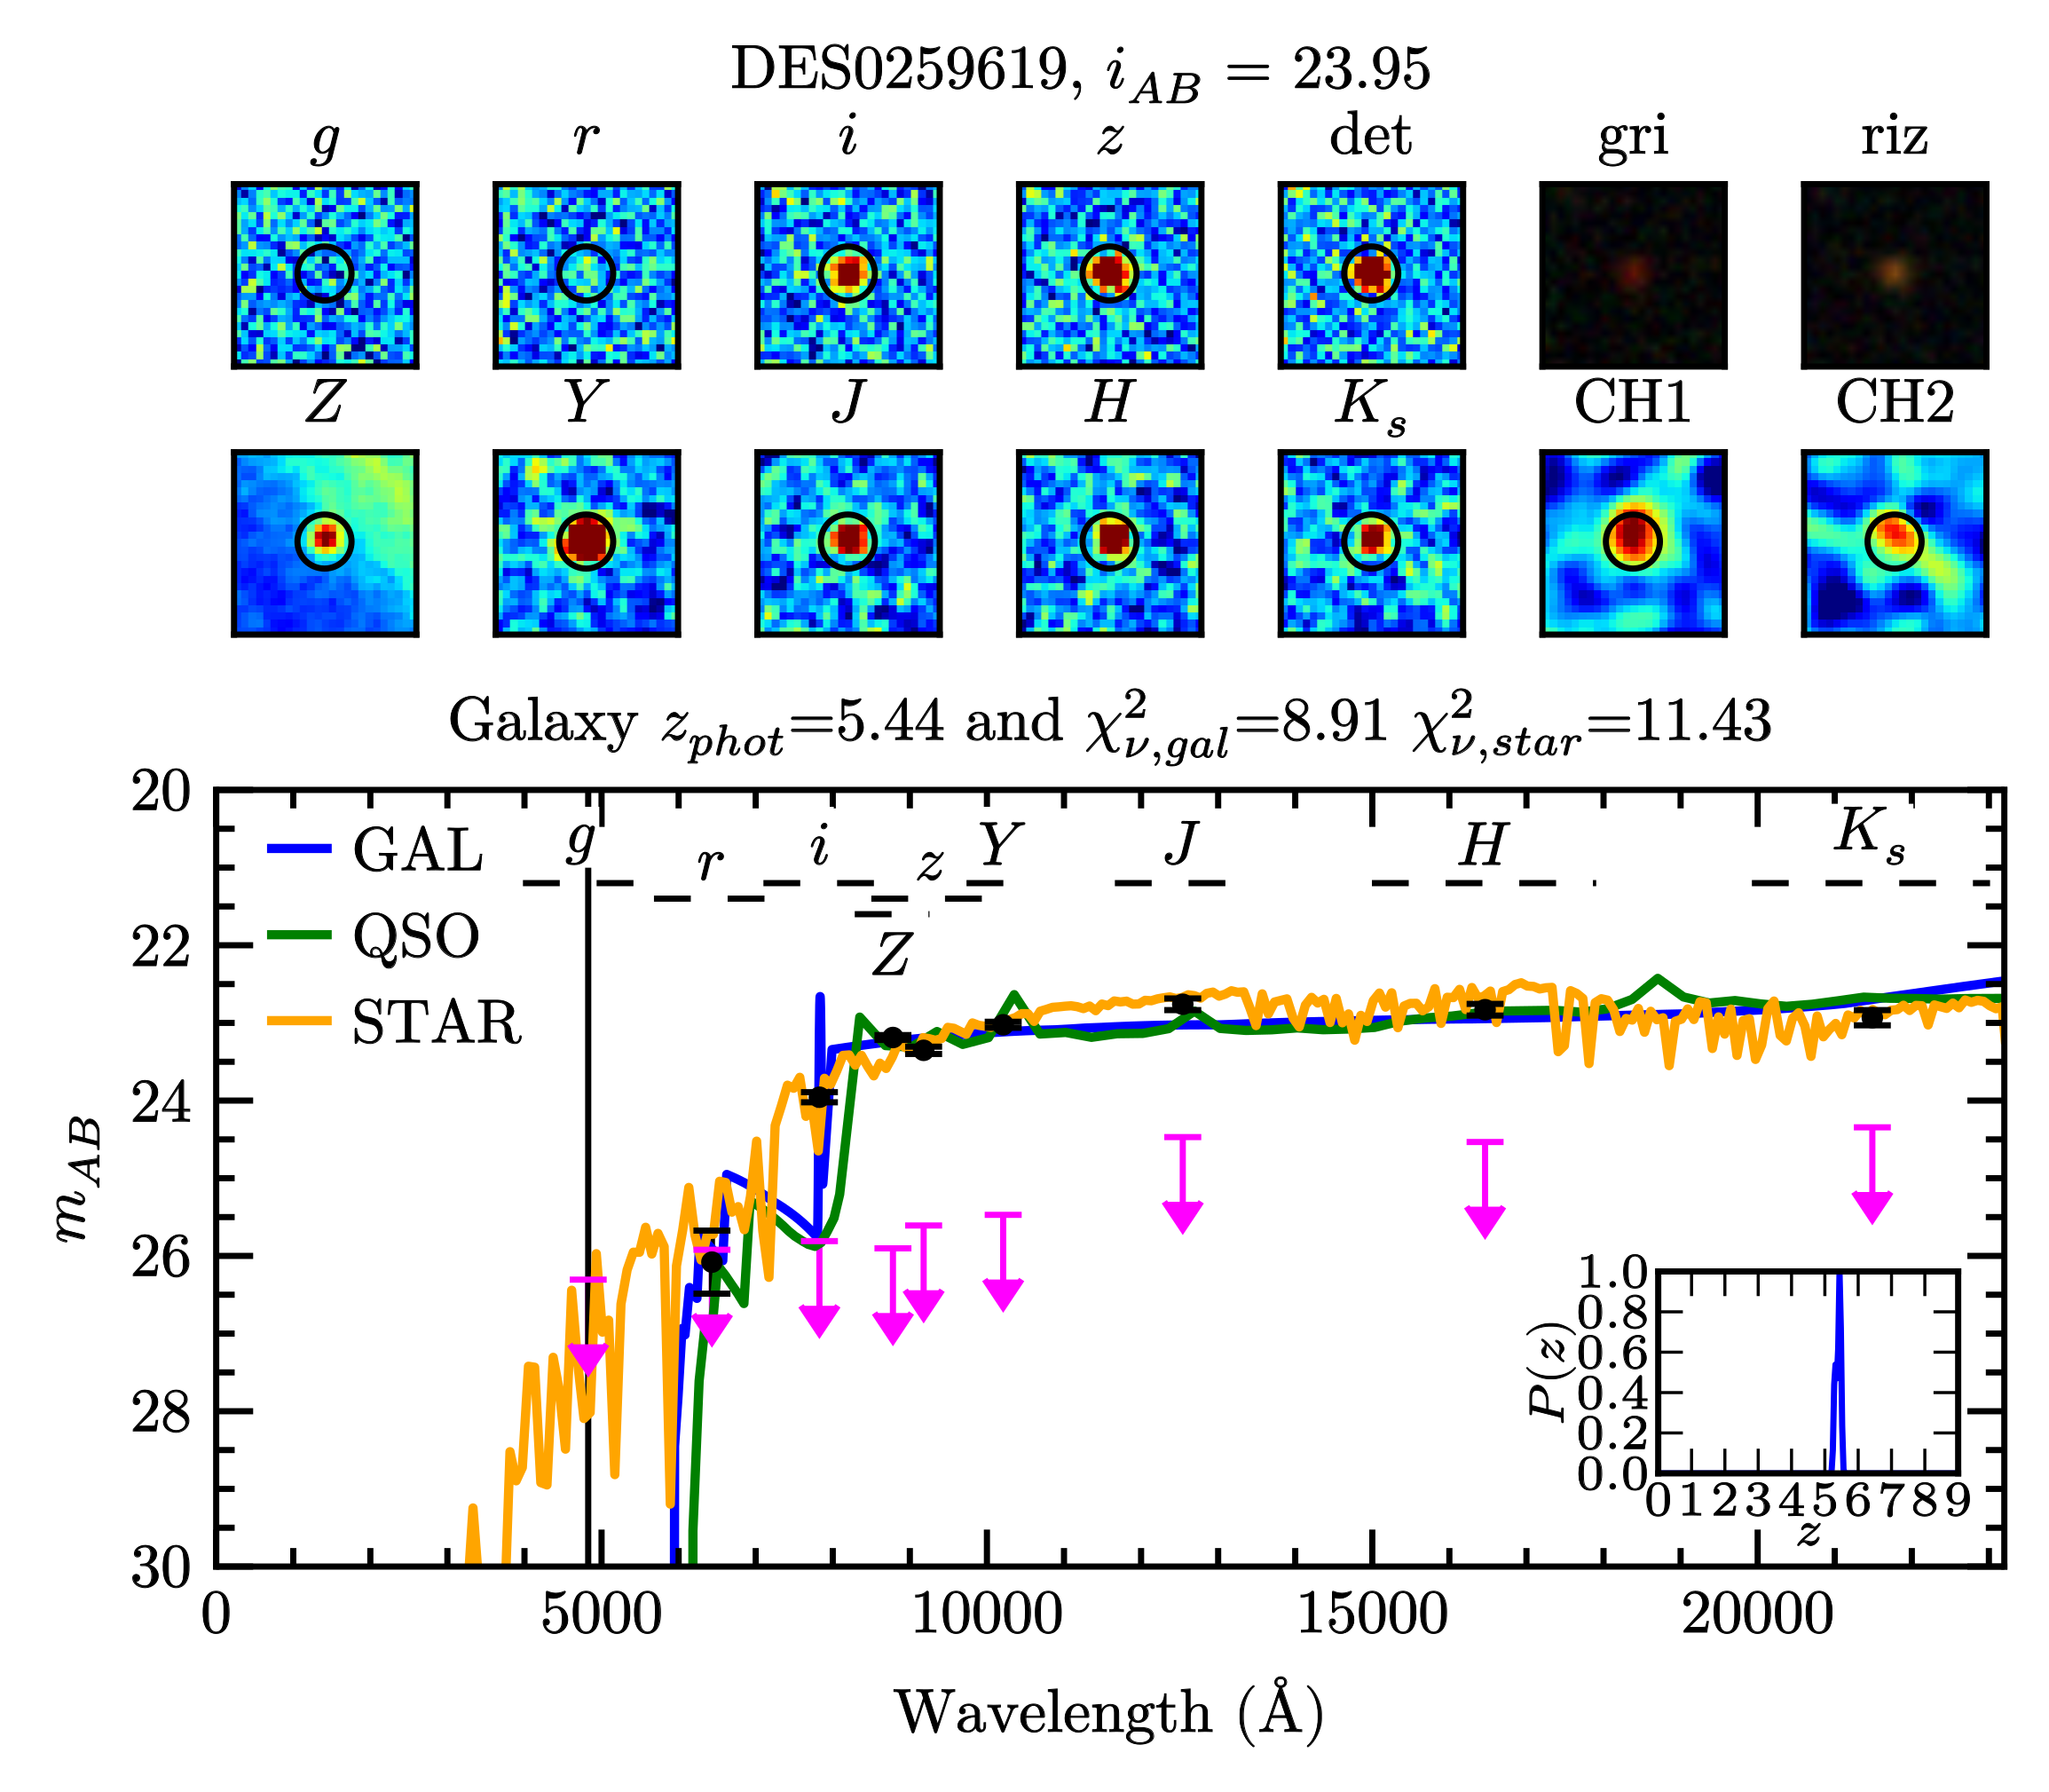
\includegraphics[width=0.95\textwidth]{Chapter4/Figs/DES0259619_thesis.png}
\caption[Example of a stellar contaminant]{An example of a suspected stellar contaminant caused by biased photometry. The postage stamps for this object indicate point source emission in all filters, which, for an object this bright ($i_{\mathrm{AB}}=23.95$) suggests that the source is likely a star. The SED plots support this hypothesis, as they show photometry that is on the whole (more) compatible with the stellar template. The high photometric redshift is likely strongly influenced by extremely small error bars in the $Z$-filter. These small uncertainties, in turn, are caused by boosting of the $Z$-band flux due to background emission from the extended PSF of a very bright star (which was discovered upon zooming out on the imaging).}
\label{fig:example_star}
\end{figure}


Stars constitute the final contaminant type that was revealed by visual inspection. Out of all the different categories of contamination, these sources were the most challenging to identify, because their inspection images contain the least distinctive features. Nevertheless, there are a few possible indicators. First of all, some stellar contaminants can in theory show blue emission, as explained during the discussion of low-redshift interlopers in Section \ref{subsubsection:contamination_low_z}. Secondly, the morphology in the postage stamps can provide some clues, since stars always appear as point sources, whereas a substantial fraction of bright galaxies are likely resolved. Unfortunately, it is expected that some of the $z\sim5$ galaxies targeted in this thesis are also unresolved in the \DESVIDEO imaging, as previously described in  Sections \ref{subsubsection:input_phot_default} and  \ref{subsubsection:star_galaxy_background}. Nonetheless, if a very bright preliminary candidate shows PSF-shaped emission in all filters, this increases the likelihood that it is a stellar contaminant. The third and most reliable indicator for finding stars, however, is their photometry. During visual inspection, it was found that some preliminary candidates have an observed SED that appears for the most part more compatible with the best-fit stellar template than the best-fit galaxy template (despite the fact that the preliminary star-galaxy separation cut required that the galaxy template has a lower $\chi^2_{\nu}$). Similarly to the analogous issue with low-redshift interlopers, this suggests the possibility of template incompleteness or inaccurate photometry. Again, it was observed that there are some cases where a high-redshift galaxy fit might be favoured due to one or two bands with very small errors, while the other bands are more compatible with a stellar fit. In other cases, the postage stamps indicate poor or biased imaging in one or more filters. In the end, it was decided to classify preliminary candidates as a potential star if they display a PSF-like morphology in all filters, and either a) they have an observed SED that appears on the whole (more) compatible with a stellar fit or b) they show an excess of blue flux (according to the requirements laid out previously in Section \ref{subsubsection:contamination_low_z}). An example of a suspected star is presented in Figure \ref{fig:example_star}. This object appears stellar in shape and shows a good fit to the stellar template in most filters, but its fit has been biased by flux from one of the rings in the extended PSF of an extremely bright nearby star. \par 



\subsection{Second round of cuts}\label{subsection:second_cuts}
After visual inspection identified the types of contamination in the preliminary sample, a series of targeted cuts was made to address each of these categories. This second selection round narrowed the sample down to a final set of secure high-redshift galaxy candidates. The following sections will describe the cuts in this final stage. \par 


\subsubsection{Artefacts and transients}
The first cut addressed artefacts and transients. Because this type of contamination was exclusively found among $z\sim6$ candidates (as discussed in Section \ref{subsubsection:contamination_transients}), this step was only applied to these objects. All transients, as well as most artefacts, only show large fluxes in one band, and artefacts that are present in multiple bands are usually only bright in some filters. Therefore, the vast majority could be removed by requiring that any final candidate must be detected to a significance of at least $3\sigma$ in a second filter redwards of the Lyman break. Bearing in mind the intrinsic blue colours of LBGs, the optimal filter for this would be the $Z$-band, but because data in this band does not exist for all VIDEO tiles, $Y$ or $J$ detections were also permitted. According to Equation \ref{eqn:sigma_m}, a $> 3\sigma$ significance corresponds to a magnitude error of $\sigma_{m}< 0.3619$, so that the cut in question amounts to the following: 

\begin{equation}
    \sigma_{Z}< 0.3619  \quad \lor \quad \sigma_{Y}< 0.3619 \quad \lor \quad \sigma_{J}< 0.3619 \qquad \text{for the } z \sim 6 \text{ sample}.
\end{equation}

\noindent After this step, there were 179 candidates left in the $z\sim6$ sample. \par 


\subsubsection{Low-redshift galaxies and QSOs}\label{subsubsection:second_round_lowz}
Contamination from low-redshift galaxies and QSOs  was tackled via a combination of five cuts that addressed the issues identified in Section \ref{subsubsection:contamination_low_z}. These cuts are listed and described below: 

\begin{itemize}
\item{} As established in Section \ref{subsubsection:contamination_low_z}, the presence of $g$-band flux is a definite indicator of contamination, most likely from low-redshift galaxies (including QSOs), or possibly from stars. To tackle such contaminants, only with objects $g$-band flux below the local $2\sigma$ magnitude limit were retained in the sample: 

\begin{equation}
    g_{\mathrm{AB}} <  m_{\mathrm{lim}, 2\sigma}
\end{equation}

\noindent This cut resulted in a total of 126 and 153 remaining objects in the $z\sim5$ and $z\sim6$ samples respectively. 

\item{} The next step targeted contaminants whose observed photometry appears overall more consistent with a low-redshift template, despite a good high-redshift $\chi^{2}_{\nu}$. When describing these objects in Section \ref{subsubsection:contamination_low_z}, it was suggested that inaccurate photometry is one of the causes of this issue. For many such low-redshift interlopers, the photometric redshift was found to be skewed towards a high-redshift result by small errors in one or more filters. To eliminate any bias from bands with very low errors, a second photo-z run was performed on all preliminary candidates, this time imposing a floor\footnote{It is interesting to note that the imposed threshold of $\sigma_{m}=0.1$ is roughly equal to the maximum adaptive offset in this thesis (see Section \ref{subsection:adaptive_offsets}), which is 0.08 in the $H$-band of the cdfs1 tile. Therefore, the error floor also insures the final candidate sample against any contamination that could result from these offsets.} on the uncertainties such that any error below $\sigma_{m}<0.1$ was increased to $\sigma_{m}=0.1$. Any candidates that switched to a low-redshift solution with these higher errors were then eliminated by imposing the following requirement:  

\begin{equation}
     z_{\mathrm{phot,high\_error}} > 4.73.\label{eqn:high_error_cut}
\end{equation}

\noindent This new redshift threshold is 0.1 lower than the previous lower bound at $z_{\mathrm{phot}}=4.83$ in order to allow for a slight shift in photometric redshift. For the same reason, objects were also permitted to swap between the $z\sim5$ or $z\sim6$ bins. After this process, there were 90 candidates left at $z\sim5$ and 115  at $z\sim6$. 



\item{} Candidates were also rejected if \texttt{LePHARE} found a secondary solution at low redshift, either with the original errors or the higher errors introduced in the previous step. Like in the previous step, `low-redshift' has been defined as $z\leq4.73$ for the purpose of this cut. Since \texttt{LePHARE} assigns a secondary redshift of $z_{\mathrm{sec}}=-99.0$ to objects without any secondary solution, the cut can be formulated as follows: 

\begin{equation}
\begin{alignedat}{1}
    (z_{\mathrm{sec}}< 0 \quad &\lor \quad z_{\mathrm{sec}}>4.73) \quad \land \quad \\ (z_{\mathrm{sec, high\_error}}< 0 \quad &\lor \quad z_{\mathrm{sec, high\_error}}>4.73).\label{eqn:z_sec_cut}
\end{alignedat}
\end{equation} 

\noindent After this step\footnote{It must be noted that the $z>4.73$ parts of the criterion turned out to be inconsequential since all secondary redshifts in the preliminary sample happen to fall below $z=2$.}, the samples contained a total of 70 and 101 candidates at $z\sim5$ and $z\sim6$ respectively. 


\item{} To remove any further low-redshift galaxy stragglers, the next step placed a restriction on the likelihood of a $z\leq 2.0$ solution. To achieve this, \texttt{LePHARE} was run for a third time in order to compute the $\chi^2_{\nu,z\leq2.0}$ value of the best possible $z\leq2.0$ galaxy solution for each candidate. This third run used the higher errors introduced above, and imposed a maximum permitted redshift of $z = 2.0$ during photo-z fitting. It was required that the resulting low-redshift solutions must be a significantly worse fit than the earlier high-redshift solutions, with the ratio set to: 

\begin{equation}
    \frac{\chi^2_{\nu,\mathrm{high\_error}}}{\chi^2_{\nu,\mathrm{high\_error},z\leq 2.0}}< 0.4. \label{eqn:low_z_cut}
\end{equation} 


\noindent The relatively restrictive threshold of 0.4 was chosen to ensure maximum purity of the final sample, so that any final candidate must have a high-redshift $\chi^2_{\nu}$ just over twice as good as the best low-redshift alternative. In the end, imposing Equation \ref{eqn:low_z_cut} did not eliminate any $z\sim5$ candidates, leaving the size of that sample at 70. The number of $z\sim6$ candidates was cut down to 95. 

\item{} Possible contamination by low-redshift quasars was addressed by removing any candidates with an acceptable low-redshift QSO solution. An acceptable fit has been defined as $\chi^2_{\nu}< 10.0$, the same threshold as in Equation \ref{eqn:galaxy_fit} of the preliminary cuts. `Low-redshift' has again been defined as  $z\leq4.73$. The requirements were applied to the QSO fits from both the original and higher errors, so that any candidate must satisfy:   

\begin{equation}
\begin{alignedat}{1}
    (z_{\mathrm{QSO}}>4.73 \quad &\lor \quad \chi^2_{\nu,\mathrm{QSO}}\geq10.0) \quad \land \quad \\ (z_{\mathrm{QSO,high\_error}}>4.73 \quad &\lor \quad \chi^2_{\nu,\mathrm{QSO,high\_error}}\geq10.0).\label{eqn:qso_cut}
\end{alignedat}
\end{equation} 

\noindent This cut did not eliminate any $z\sim5$ objects, leaving 70 candidates in that sample. For the $z\sim6$ sample, 87 objects remained. 
\end{itemize}

\subsubsection{Stars}
Contamination from stars is the last major issue that had to be confronted. As explained in Section \ref{subsubsection:contamination_stars}, visual inspection indicated that the SEDs for many of these potential stellar contaminants appear more compatible with a star than galaxy templates in most filters, an issue also noted among low-redshift interlopers. Similarly, inaccurate photometry was identified as a likely cause. Therefore, contamination from stars was addressed by imposing a second star-galaxy separation criterion, this time using the aforementioned higher photometric errors. Analogous to the low-redshift equivalent in Equation \ref{eqn:low_z_cut}, this cut consists of a maximum on the ratio between the star and galaxy $\chi^2_{\nu,\mathrm{high\_error}}$: 

\begin{equation}
    \frac{\chi^2_{\nu,\mathrm{gal,high\_error}}}{\chi^2_{\nu,\mathrm{star,high\_error}}}< 0.4. \label{eqn:second_star_cut}
\end{equation}

\noindent After this step, there were 39 and 54 candidates left in the $z\sim5$ and $z\sim6$ samples respectively.  \par

\subsubsection{Manual removal}
Despite the specialised cuts described so far, at this point the $z\sim6$ sample still contained 13 contaminants. Among these are 10 imaging artefacts and transient objects that accurately replicate high-redshift SEDs, for instance because they overlap with a true object, or with diffuse background flux from e.g. bright stars. The other 3 contaminants contain $g$-band imaging in a noisy region around the chip gaps, so that their dropout behaviour could not be reliably confirmed. All these 13 sources were removed from the sample by hand. This final step narrowed the $z\sim6$ sample down to 41 objects. \par



\subsubsection{Summary and verification of the second selection round}\label{subsubsection:verification_second_round}
The second round of cuts described in the preceding sections has thus resulted in a final sample of 39 $z\sim5$ and 41 $z\sim6$ candidates. Table \ref{table:final_cuts} summarises this round by listing all the selection steps that have been applied. \par 

%The end result of the second round of cuts is thus a final sample of x candidates. To summarise this round, Table x presents an overview of all the selection steps

%To summarise, the end result of the second round of cuts is a final sample of 39 $z\sim5$ and 41 $z\sim6$ candidates. Table \ref{table:final_cuts} presents an overview of this process, listing all the selection steps that were applied. 
%The cuts in the previous sections describing the second round have thus produced...


%The previous section concludes the second round of cuts. To summarise, the resulting final sample consists of 39 $z\sim5$, and 41 $z\sim6$ candidates, and all the selection steps are listed in Table \ref{table:final_cuts}. To investigate the effectiveness of these cuts, it is important to verify their effect on sample purity and completeness. Regarding purity, the inspection images of all the final candidates reassuringly indicate no signs of contamination in both the $z\sim5$ and $z\sim6$ samples. This suggests that the aim of isolating a highly secure sample of high-redshift galaxies {\color{red}is} successful. The completeness part of the verification procedure, assesses the inspection images of all the objects rejected at each step of the second round, to check whether any of them could be real high-redshift galaxies. The remainder of this section describes the results of this process. 

\afterpage{
\clearpage
\begin{table}[p]
\centering
\begin{ThreePartTable}
\setlength{\tabcolsep}{0.1em}
\textsc{Candidate Cuts} \\
\vspace{0.2em}
\begin{tabular}{lcclc}
\toprule
\multicolumn{2}{c}{\textsc{$z\sim5$ sample}} & & \multicolumn{2}{c}{\textsc{$z\sim6$ sample}}  \\
%\cmidrule{1-2} & & \cmidrule{4-5}\\
%\toprule\toprule
cut definition & remaining & \hspace{1.5em} & cut definition & remaining \\ 
\toprule\toprule 
\vspace{-0.8em}\\
%\doublespacing
Preliminary sample & 131 & & Preliminary sample & 320 \\ \midrule

--- & 131 & &   \begin{tabular}{@{}l@{}}$\sigma_{Z}< 0.3619 \thickspace\thickspace\thickspace \lor $ \\ \hspace{0.2em} $\sigma_{Y}< 0.3619$ \lor  \\ \hspace{0.2em} $\sigma_{J}< 0.3619$ \end{tabular}  & 179 \vspace{0.4em} \\

$g_{\mathrm{AB}} <  m_{\mathrm{lim}, 2\sigma}$ & 126 & & $g_{\mathrm{AB}} <  m_{\mathrm{lim}, 2\sigma}$ & 153 \vspace{0.4em} \\

$z_{\mathrm{phot, high\_error}} > 4.73$ & 90 & & $z_{\mathrm{phot, high\_error}} > 4.73$ & 115 \vspace{0.4em} \\

%$z_{\mathrm{sec}}< 0  \land z_{\mathrm{sec}, high\_error}< 0$ & 70 & & $z_{\mathrm{sec}}< 0  \land z_{\mathrm{sec}, high\_error}< 0$ & 101  \vspace{0.4em}\\

\begin{tabular}{@{}l@{}} $(z_{\mathrm{sec}}< 0$ \thickspace \lor \thickspace $z_{\mathrm{sec}}>4.73)$ \thickspace \land \\   \hspace{0.2em} $(z_{\mathrm{sec, high\_error}}< 0$ \lor \\  \hspace{0.2em} \thickspace $z_{\mathrm{sec,high\_error}}>4.73$) \end{tabular} & 70 & & \begin{tabular}{@{}l@{}} $(z_{\mathrm{sec}}< 0$ \thickspace \lor \thickspace $z_{\mathrm{sec}}>4.73)$ \thickspace \land \\   \hspace{0.2em} $(z_{\mathrm{sec,high\_error}}< 0$ \lor \\  \hspace{0.2em} \thickspace $z_{\mathrm{sec,high\_error}}>4.73$) \end{tabular} & 101 \vspace{0.4em} \\


$\frac{\chi^2_{\nu,\mathrm{gal,high\_error}}}{\chi^2_{\nu,\mathrm{high\_error},z\leq2.0}}< 0.4$ & 70 &  & $\frac{\chi^2_{\nu,\mathrm{gal,high\_error}}}{\chi^2_{\nu,\mathrm{high\_error},z\leq2.0}}< 0.4$ & 95 \vspace{0.4em} \\


\begin{tabular}{@{}l@{}} $(z_{\mathrm{QSO}}>4.73$ \lor \\ \hspace{0.2em} $\chi^2_{\nu,\mathrm{QSO}}\geq10.0)$ \land \\   \hspace{0.2em} $(z_{\mathrm{QSO,high\_error}}>4.73$ \lor \\  \hspace{0.2em} \thickspace $\chi^2_{\nu,\mathrm{QSO,high\_error}}\geq10.0)$ \end{tabular} & 70 & & \begin{tabular}{@{}l@{}} $(z_{\mathrm{QSO}}>4.73$ \lor \\ \hspace{0.2em} $\chi^2_{\nu,\mathrm{QSO}}\geq10.0)$ \land \\   \hspace{0.2em} $(z_{\mathrm{QSO,high\_error}}>4.73$ \lor \\  \hspace{0.2em} \thickspace $\chi^2_{\nu,\mathrm{QSO,high\_error}}\geq10.0)$ \end{tabular} & 87 \vspace{0.4em} \\

%$\chi^2_{\nu,high\_error}/ \chi^2_{\nu,high\_error,z< 2.0}< 0.4$ & 70 &  & $\chi^2_{\nu,high\_error}/ \chi^2_{\nu,high\_error,z< 2.0}< 0.4$ & 87 \\

$\frac{\chi^2_{\nu,\mathrm{gal,high\_error}}}{\chi^2_{\nu,\mathrm{star,high\_error}}}< 0.4$ & 39 & & $\frac{\chi^2_{\nu,\mathrm{gal,high\_error}}}{\chi^2_{\nu,\mathrm{star,high\_error}}}< 0.4$ & 54 \vspace{0.4em} \\


%$\chi^2_{\nu,gal,high\_error}/\chi^2_{\nu,star,high\_error}< 0.4$ & 39 & & $\chi^2_{\nu,gal,high\_error}/\chi^2_{\nu,star,high\_error}< 0.4$ & 54 \\

--- & 39 & & Manual removal & 41 \vspace{0.4em}\\ 


\bottomrule
\end{tabular}
\vspace{1em}
%\begin{tablenotes}
%\singlespacing
%\setstretch{0.9}\small
%\item[i] 
%\end{tablenotes}
%\vspace{1em}
\caption[Selection criteria for the second round of cuts]{An overview of the selection criteria that have been applied to the preliminary subsample to produce a final sample of high-redshift galaxy candidates. The samples of 39 $z\sim5$ and 41 $z\sim6$ candidates each contain five duplicates (see Section \ref{section:final_sample}), so there are 34 and 36 unique candidates respectively.}\label{table:final_cuts}
\end{ThreePartTable}
\end{table}
\clearpage
}





To investigate the effectiveness of these cuts, the author has investigated the completeness and purity of the sample via the inspection images. Regarding purity, the inspection images of all the final candidates reassuringly indicate no signs of contamination in both the $z\sim5$ and $z\sim6$ samples. This suggests that this thesis has succeeded in its aim of isolating a highly secure sample of high-redshift galaxies. The completeness part of the verification procedure assessed the inspection images of all the objects rejected at each step of the second round, to check whether any of them could be real high-redshift galaxies. The remainder of this section describes the results of this completeness check.  \par


For the $z\sim6$ sample, the selection proved highly successful. Most of the rejected objects are either artefacts, transients, or low-redshift galaxies. In fact, with the exception of the cut in Equation \ref{eqn:second_star_cut}, none of the steps removed preliminary candidates that would not have been rejected in a subsequent step. Equation \ref{eqn:second_star_cut} did, due to their adequate stellar fits, remove three objects which in reality cannot be stars, because their postage stamps indicate extended emission\footnote{These objects also have high values of \texttt{spread\_model}, exceeding the galaxy threshold of \texttt{spread\_model}>0.0028 posited by  \cite{2015MNRAS.446.2523B} for another DES dataset.}. It is therefore possible that these sources may be true high-redshift galaxies. However, because their photometry is not accurate enough to indicate a strong preference for a galaxy template over a stellar SED, the fit for these candidates was considered too unreliable. \par 


The selection for the $z\sim5$ sample was found to be slightly less efficient than at $z\sim5$, with some cuts removing probable real $z\sim5$ galaxies. The photometry of these rejected preliminary candidates shows a strong \SI{1216}{\angstrom} break as well as blue continuum colours, both of which are incompatible with the gently sloping red SEDs of dusty low-redshift galaxies. In many cases the postage stamps also display extended emission, ruling out a stellar origin as well. It is postulated that this unnecessary rejection, which did not occur in the $z\sim6$ sample, is partly caused by the minimum $\sigma_{m}>0.1$ error floor (introduced in Section \ref{subsubsection:second_round_lowz} and used in Equations \ref{eqn:high_error_cut}, \ref{eqn:z_sec_cut}, \ref{eqn:low_z_cut}, \ref{eqn:qso_cut}, and \ref{eqn:second_star_cut}). Because the magnitude uncertainty $\sigma_{m}$ scales proportionally with the flux uncertainty $\sigma_{F}$ and inversely with the flux $F$ (see Equation \ref{eqn:sigma_m}), this error floor only affects filters with sufficiently deep data and adequately bright emission. Galaxies at $z\sim5$ are on average brighter than their $z\sim6$ counterparts in all filters, and they are also bright in more filters, since they emit (rest-frame UV) continuum flux in both the $i$- and $z$-band rather than the $z$-band alone. Emission from the $i$-band is comparatively more affected by the error floor, because this filter is deeper than the $z$-band and VIDEO bands. On the whole, all these factors entail that the imposition of minimum errors has a larger effect on the $z\sim5$ photometry. This effect could lead to the rejection of real candidates, because the higher errors produce a lower $\chi^2_{\nu}$ for all templates, increasing the possibility of a low-redshift secondary solution, as well as the likelihood of a low-redshift primary solution (due to the prior vastly favouring low-redshift fits). In addition to the error floor, another potential cause for the removal of probable $z\sim5$ candidates is that the second round of cuts has been made conservative by design. Strong cuts have been chosen in order to reduce contamination, which could come at the cost of rejecting some true candidates. This issue affects the $z\sim5$ sample more strongly, because $z\sim5$ galaxies are more compatible with a larger range of star and low-redshift galaxy templates, due to dropout behaviour being displayed in one fewer filter. As a result, $z\sim5$ fits may be less likely to pass the conservative second round cuts. One could argue that the use of the higher errors is therefore not appropriate at $z\sim5$. However, it was found that several stellar and low-redshift contaminants enter the final sample when the error floor is removed. It was therefore decided to retain the minimum errors, in order to ensure a maximally secure sample. An additional advantage of this decision is that it also enables a more direct comparison with the $z\sim6$ candidates. Nevertheless, it would be interesting to investigate whether it would be possible to formulate alternative selection criteria for the $z\sim5$ sample that reject fewer good candidates. This task is left as a suggestion for future work. \par 


\section{Final sample}\label{section:final_sample}

\afterpage{\clearpage
\begin{ThreePartTable}
\centering
\onehalfspacing
\footnotesize

\begin{TableNotes}
%\vspace{-0.2em}
\onehalfspacing
\textbf{Notes:}\\
The sample contains five pairs of duplicates, originating from the tile overlap listed below. The parentheses after each tile enclose the catalogue ID of the duplicate object in that tile.\\
\item[a] Duplicates from the es1-north (DES0261588) and es1-south (DES0334028) VIDEO tiles. \\
\item[b] Duplicates from the DES0236-2832 (DES1429846) and DES0328-2749 (DES1613457) DES tiles. \\
\item[c] Duplicates from the cdfs1 (DES1480785) and cdfs2 (DES1615885) VIDEO tiles. \\
\item[d] Duplicates from the DES0328-2749 (DES1513918) and DES0332-2749 (DES1873583) DES tiles. \\
\item[e] Duplicates from the DES0332-2832 (DES2022830) and DES03333-2915 (DES2191223) DES tiles. \\
\vspace{0.5em}
\end{TableNotes}

%\renewcommand\TPTminimum{\textwidth}
\setlength{\tabcolsep}{0.4em}
%\setlength\LTleft{-1.7cm}
%\setlength\LTright{1.7cm}
\centering
%\small
\doublespacing
\begin{longtable}{lccccccl}
\multicolumn{8}{c}{\textsc{$z\sim5$ Candidate Sample}}\\
\toprule\toprule 
ID & RA and Dec (J2000) & $\thickspace z_{\mathrm{phot}} \thickspace$ & $r_{\mathrm{AB}}$ & $i_{\mathrm{AB}}$ & $z_{\mathrm{AB}}$ & $J_{\mathrm{AB}}$ & Notes \\
\midrule
\endfirsthead
\multicolumn{8}{c}{\normalsize \textsc{$z\sim5$ Candidate Sample (continued)}}\\
\toprule\toprule 
ID & RA and Dec (J2000) & $\thickspace z_{\mathrm{phot}} \thickspace$ & $r_{\mathrm{AB}}$ & $i_{\mathrm{AB}}$ & $z_{\mathrm{AB}}$ & $J_{\mathrm{AB}}$ & Notes \\
\midrule
\endhead
\bottomrule
\multicolumn{8}{r}{\textit{continued}}
\endfoot
\midrule\midrule
\insertTableNotes \\
\bottomrule \\
\caption[Final \texorpdfstring{$z\sim5$}{} candidate sample]{The final sample of $z\sim5$ candidates, with for each candidate its catalogue ID, position, photometric redshift $z_{\mathrm{phot}}$, and $r$-, $i$-, $z$-, and $J$-band magnitude. The sample contains five pairs of duplicates, which are flagged in the notes. The value of $z_{\mathrm{phot}}$ is the photometric redshift computed with the original uncertainties (i.e. without the error floor imposed in Section \ref{subsubsection:second_round_lowz}). Magnitudes are given for a \SI{1.95}{\arcsec} diameter aperture. If the magnitude of a candidate falls below the $1\sigma$ depth in that area, the $1\sigma$ limiting magnitude is shown instead.}\label{table:candidates_5}\\
\endlastfoot


DES0261588 & 00:40:13.35-44:00:37.26 & 5.03 & $25.15^{ \pm 0.18}$ & $23.41^{ \pm 0.04}$ & $22.99^{ \pm 0.04}$ & $23.25^{ \pm 0.12}$ & \tnote{a} \\
DES0334028 & 00:40:13.35-44:00:37.26 & 4.98 & $25.15^{ \pm 0.18}$ & $23.41^{ \pm 0.04}$ & $22.99^{ \pm 0.04}$ & $23.20^{ \pm 0.11}$ & \tnote{a} \\
DES0773209 & 02:22:28.00-04:51:37.10 & 4.95 & $> 28.24$ & $25.00^{ \pm 0.06}$ & $24.67^{ \pm 0.05}$ & $24.94^{ \pm 0.30}$ & \\
DES0892423 & 02:24:43.46-04:33:16.77 & 4.98 & $26.97^{ \pm 0.33}$ & $24.89^{ \pm 0.05}$ & $24.61^{ \pm 0.05}$ & $24.84^{ \pm 0.27}$ & \\
DES0924984 & 02:25:10.25-04:12:22.94 & 4.97 & $26.19^{ \pm 0.18}$ & $24.57^{ \pm 0.04}$ & $24.29^{ \pm 0.04}$ & $24.63^{ \pm 0.22}$ & \\
DES0927703 & 02:25:17.30-04:10:47.95 & 4.88 & $26.32^{ \pm 0.20}$ & $24.73^{ \pm 0.04}$ & $24.57^{ \pm 0.05}$ & $24.59^{ \pm 0.22}$ & \\
DES1008140 & 02:23:39.65-04:38:34.73 & 4.96 & $26.53^{ \pm 0.23}$ & $24.68^{ \pm 0.05}$ & $24.46^{ \pm 0.04}$ & $24.58^{ \pm 0.22}$ & \\
DES1027267 & 02:25:31.35-05:10:25.29 & 4.90 & $27.06^{ \pm 0.36}$ & $24.87^{ \pm 0.05}$ & $24.83^{ \pm 0.06}$ & $25.25^{ \pm 0.40}$ & \\
DES1053297 & 02:25:18.60-04:57:41.88 & 4.90 & $27.28^{ \pm 0.45}$ & $24.87^{ \pm 0.06}$ & $24.61^{ \pm 0.05}$ & $24.68^{ \pm 0.23}$ & \\
DES1069344 & 02:24:26.12-04:49:48.35 & 5.04 & $26.33^{ \pm 0.19}$ & $24.92^{ \pm 0.06}$ & $24.53^{ \pm 0.05}$ & $24.73^{ \pm 0.25}$ & \\
DES1099438 & 02:24:23.91-05:28:06.61 & 4.90 & $26.03^{ \pm 0.16}$ & $24.33^{ \pm 0.03}$ & $24.09^{ \pm 0.03}$ & $24.11^{ \pm 0.14}$ & \\
DES1158545 & 02:27:55.10-04:23:57.81 & 4.89 & $27.12^{ \pm 0.40}$ & $24.82^{ \pm 0.05}$ & $24.72^{ \pm 0.06}$ & $24.56^{ \pm 0.21}$ & \\
DES1230744 & 02:28:01.00-03:59:37.89 & 4.88 & $26.26^{ \pm 0.15}$ & $24.49^{ \pm 0.03}$ & $24.36^{ \pm 0.03}$ & $24.18^{ \pm 0.15}$ & \\
DES1240477 & 02:28:02.95-05:17:21.98 & 4.97 & $27.07^{ \pm 0.37}$ & $24.86^{ \pm 0.05}$ & $24.56^{ \pm 0.05}$ & $24.74^{ \pm 0.25}$ & \\
DES1248943 & 02:27:26.10-05:13:47.74 & 4.91 & $27.11^{ \pm 0.38}$ & $24.65^{ \pm 0.04}$ & $24.45^{ \pm 0.04}$ & $24.38^{ \pm 0.18}$ & \\
DES1266621 & 02:28:40.91-05:08:12.87 & 5.01 & $25.92^{ \pm 0.13}$ & $24.44^{ \pm 0.04}$ & $24.09^{ \pm 0.03}$ & $24.48^{ \pm 0.19}$ & \\
DES1391206 & 03:26:57.50-27:47:26.78 & 4.89 & $26.70^{ \pm 0.21}$ & $24.49^{ \pm 0.04}$ & $24.58^{ \pm 0.04}$ & $24.62^{ \pm 0.23}$ & \\
DES1429846 & 03:27:26.41-28:11:04.15 & 5.03 & $26.28^{ \pm 0.14}$ & $24.59^{ \pm 0.04}$ & $24.23^{ \pm 0.03}$ & $24.36^{ \pm 0.26}$ & \tnote{b} \\
DES1453274 & 03:29:25.84-27:19:34.34 & 4.89 & $26.10^{ \pm 0.12}$ & $24.47^{ \pm 0.04}$ & $24.30^{ \pm 0.03}$ & $24.43^{ \pm 0.19}$ &  \\
DES1480785 & 03:30:09.41-28:10:13.10 & 4.86 & $25.40^{ \pm 0.06}$ & $23.93^{ \pm 0.02}$ & $23.75^{ \pm 0.02}$ & $23.75^{ \pm 0.10}$ & \tnote{c} \\
DES1506707 & 03:29:09.48-28:01:35.17 & 5.29 & $26.75^{ \pm 0.22}$ & $24.81^{ \pm 0.05}$ & $24.17^{ \pm 0.03}$ & $24.20^{ \pm 0.16}$ & \\
DES1510338 & 03:30:21.63-28:00:28.02 & 4.97 & $26.36^{ \pm 0.15}$ & $24.66^{ \pm 0.04}$ & $24.39^{ \pm 0.03}$ & $24.65^{ \pm 0.24}$ & \\
DES1513918 & 03:30:29.44-27:59:21.69 & 4.91 & $26.87^{ \pm 0.25}$ & $24.96^{ \pm 0.05}$ & $24.82^{ \pm 0.05}$ & $25.19^{ \pm 0.39}$ & \tnote{d} \\
DES1516307 & 03:28:44.72-27:58:41.09 & 5.29 & $27.15^{ \pm 0.32}$ & $24.98^{ \pm 0.06}$ & $24.38^{ \pm 0.03}$ & $24.68^{ \pm 0.24}$ & \\
DES1613457 & 03:27:26.41-28:11:04.15 & 5.02 & $26.28^{ \pm 0.14}$ & $24.58^{ \pm 0.04}$ & $24.22^{ \pm 0.03}$ & $24.31^{ \pm 0.25}$ & \tnote{b} \\
DES1615885 & 03:30:09.41-28:10:13.10 & 4.84 & $25.40^{ \pm 0.06}$ & $23.93^{ \pm 0.02}$ & $23.75^{ \pm 0.02}$ & $23.74^{ \pm 0.15}$ & \tnote{c} \\
DES1683336 & 03:29:18.72-28:40:21.16 & 4.88 & $26.76^{ \pm 0.22}$ & $24.77^{ \pm 0.04}$ & $24.50^{ \pm 0.04}$ & $24.59^{ \pm 0.32}$ & \\
DES1798803 & 03:30:27.12-27:19:41.66 & 4.88 & $26.71^{ \pm 0.22}$ & $24.91^{ \pm 0.05}$ & $24.69^{ \pm 0.05}$ & $24.61^{ \pm 0.23}$ & \\
DES1802305 & 03:32:45.06-27:18:38.68 & 4.89 & $26.82^{ \pm 0.24}$ & $24.95^{ \pm 0.06}$ & $24.78^{ \pm 0.05}$ & $24.88^{ \pm 0.29}$ & \\
DES1870784 & 03:30:54.31-28:00:20.08 & 4.83 & $25.88^{ \pm 0.10}$ & $24.34^{ \pm 0.03}$ & $24.34^{ \pm 0.03}$ & $24.34^{ \pm 0.18}$ & \\
DES1873583 & 03:30:29.44-27:59:21.77 & 4.91 & $26.89^{ \pm 0.26}$ & $24.96^{ \pm 0.05}$ & $24.84^{ \pm 0.05}$ & $25.07^{ \pm 0.35}$ & \tnote{d} \\
DES1929684 & 03:30:54.69-27:39:17.44 & 4.96 & $26.67^{ \pm 0.21}$ & $24.79^{ \pm 0.05}$ & $24.54^{ \pm 0.04}$ & $24.50^{ \pm 0.21}$ & \\
DES1941550 & 03:32:54.04-27:34:44.68 & 4.97 & $26.72^{ \pm 0.21}$ & $24.70^{ \pm 0.04}$ & $24.47^{ \pm 0.04}$ & $24.41^{ \pm 0.19}$ & \\
DES2022830 & 03:32:07.78-28:53:22.34 & 4.84 & $25.65^{ \pm 0.08}$ & $24.21^{ \pm 0.03}$ & $23.96^{ \pm 0.02}$ & $24.15^{ \pm 0.21}$ & \tnote{e} \\
DES2023522 & 03:32:41.96-28:53:06.73 & 4.96 & $26.58^{ \pm 0.19}$ & $24.49^{ \pm 0.04}$ & $24.11^{ \pm 0.03}$ & $24.05^{ \pm 0.19}$ & \\
DES2048158 & 03:31:36.51-28:43:14.73 & 5.28 & $26.73^{ \pm 0.21}$ & $24.91^{ \pm 0.05}$ & $24.27^{ \pm 0.03}$ & $24.04^{ \pm 0.19}$ & \\
DES2122745 & 03:31:45.95-28:12:02.69 & 4.95 & $26.99^{ \pm 0.24}$ & $24.83^{ \pm 0.07}$ & $24.75^{ \pm 0.05}$ & $25.08^{ \pm 0.50}$ & \\
DES2177455 & 03:31:32.36-29:01:48.78 & 4.96 & $26.94^{ \pm 0.28}$ & $24.45^{ \pm 0.03}$ & $24.08^{ \pm 0.02}$ & $24.05^{ \pm 0.19}$ & \\
DES2191223 & 03:32:07.78-28:53:22.21 & 4.83 & $25.63^{ \pm 0.08}$ & $24.20^{ \pm 0.03}$ & $23.95^{ \pm 0.02}$ & $24.14^{ \pm 0.21}$ & \tnote{e} \\


\end{longtable}
\end{ThreePartTable}

\clearpage

\begin{ThreePartTable}
\centering
\onehalfspacing
\footnotesize

\begin{TableNotes}[]
\onehalfspacing
\textbf{Notes:}\\
The sample contains five pairs of duplicates, originating from the tile overlap listed below. The parentheses after each tile  enclose the catalogue ID of the duplicate object in that tile.\\
\item[a] Duplicates from the DES0221-0416 (DES0688180) and DES0223-0416 (DES0826107) DES tiles. \\
\item[b] Duplicates from the xmm2 (DES0853065) and xmm3 (DES0911243) VIDEO tiles. \\
\item[c] Duplicates from the xmm2 (DES0975555) and xmm3 (DES1049468) VIDEO tiles. \\
\item[d] Duplicates from the DES0328-2706 (DES1431780) and DES0328-2749 (DES1611505) DES tiles. \\
\item[e] Duplicates from the cdfs1 (DES1494058) and cdfs2 (DES1627764) tiles. \\
\vspace{-0.7em} \\
Three candidates correspond to the following objects from a sample by  \cite{2013AJ....145....4W}: \\
\item[f] WMH2 \\
\item[g] WMH3 \\
\item[h] WMH5 \\
\vspace{-0.7em} \\
Spectroscopy:\\
\item[i] Candidate selected for spectroscopic follow-up. \\
\vspace{0.5em}
\end{TableNotes}

\renewcommand\TPTminimum{\textwidth}
\setlength{\tabcolsep}{0.4em}
%\setlength\LTleft{-1.7cm}
%\setlength\LTright{1.7cm}
%\centering
%\footnotesize
\doublespacing
\begin{longtable}{lccccccl}
\multicolumn{8}{c}{\textsc{$z\sim6$ Candidate Sample}}\\
\toprule\toprule 
ID & RA and Dec (J2000) & $\thickspace z_{\mathrm{phot}} \thickspace$ & $r_{\mathrm{AB}}$ & $i_{\mathrm{AB}}$ & $z_{\mathrm{AB}}$ & $J_{\mathrm{AB}}$ & Notes \\
\midrule
\endfirsthead
\multicolumn{8}{c}{\normalsize \textsc{$z\sim6$ Candidate Sample (continued)}}\\
\toprule\toprule 
ID & RA and Dec (J2000) & $\thickspace z_{\mathrm{phot}} \thickspace$ & $r_{\mathrm{AB}}$ & $i_{\mathrm{AB}}$ & $z_{\mathrm{AB}}$ & $J_{\mathrm{AB}}$ & Notes \\
\midrule
\endhead
\bottomrule
\multicolumn{8}{r}{\textit{continued}}
\endfoot
\midrule\midrule
\insertTableNotes \\
\bottomrule \\
\caption[Final \texorpdfstring{$z\sim6$}{} candidate sample]{The final sample of $z\sim6$ candidates, with for each candidate its catalogue ID, position, photometric redshift $z_{\mathrm{phot}}$, and $r$-, $i$-, $z$-, and $J$-band magnitude.  The sample contains five pairs of duplicates, which are flagged in the notes. Objects that were found in a $z\approx6$ study by \cite{2013AJ....145....4W} are also flagged, as well as the three candidates that were submitted for spectroscopic follow-up. Further details on $z_{\mathrm{phot}}$ and the magnitude measurements are identical to those in Table \ref{table:candidates_5}.  }\label{table:candidates_6}\\
\endlastfoot


DES0027723 & 00:34:29.87-43:43:19.09 & 5.93 & $> 27.62$ & $26.86^{ \pm 0.70}$ & $24.69^{ \pm 0.11}$ & $25.21^{ \pm 0.72}$ & \\
DES0688180 & 02:22:28.32-04:33:08.94 & 5.88 & $> 28.22$ & $26.49^{ \pm 0.25}$ & $24.76^{ \pm 0.06}$ & $24.79^{ \pm 0.26}$ & \tnote{a} \\
DES0825517 & 02:23:00.37-04:33:25.15 & 6.09 & $> 28.29$ & $> 28.14$ & $24.84^{ \pm 0.06}$ & $24.76^{ \pm 0.26}$ & \\
DES0826107 & 02:22:28.33-04:33:08.91 & 5.88 & $> 28.22$ & $26.41^{ \pm 0.23}$ & $24.75^{ \pm 0.06}$ & $24.77^{ \pm 0.26}$ & \tnote{a} \\
DES0837948 & 02:23:00.03-04:27:56.15 & 5.99 & $> 28.29$ & $27.69^{ \pm 0.72}$ & $25.00^{ \pm 0.07}$ & $24.95^{ \pm 0.30}$ & \\
DES0853065 & 02:24:15.10-04:20:47.05 & 6.08 & $> 28.25$ & $> 28.14$ & $24.96^{ \pm 0.07}$ & $25.61^{ \pm 0.56}$ & \tnote{b,} \enspace \tnote{f} \\
DES0911243 & 02:24:15.10-04:20:47.05 & 6.07 & $> 28.25$ & $> 28.14$ & $24.96^{ \pm 0.07}$ & $25.02^{ \pm 0.32}$ & \tnote{b,} \enspace \tnote{f} \\
DES0938949 & 02:24:51.15-04:03:29.42 & 6.07 & $> 28.23$ & $> 28.12$ & $24.78^{ \pm 0.06}$ & $24.83^{ \pm 0.27}$ & \tnote{g,} \enspace \tnote{i} \\
DES0975555 & 02:23:52.26-04:59:27.69 & 5.90 & $27.94^{ \pm 0.82}$ & $27.15^{ \pm 0.46}$ & $24.85^{ \pm 0.06}$ & $24.75^{ \pm 0.25}$ & \tnote{c} \\
DES1020121 & 02:25:43.56-05:16:02.62 & 6.18 & $> 28.22$ & $> 28.08$ & $24.98^{ \pm 0.09}$ & $24.93^{ \pm 0.30}$ & \\
DES1026848 & 02:25:15.61-05:10:36.95 & 5.56 & $27.72^{ \pm 0.66}$ & $25.65^{ \pm 0.11}$ & $24.66^{ \pm 0.05}$ & $24.55^{ \pm 0.21}$ & \\
DES1049468 & 02:23:52.26-04:59:27.69 & 5.92 & $27.94^{ \pm 0.82}$ & $27.15^{ \pm 0.46}$ & $24.85^{ \pm 0.06}$ & $25.23^{ \pm 0.39}$ & \tnote{c} \\
DES1170574 & 02:26:55.55-04:20:05.77 & 5.85 & $> 28.29$ & $26.70^{ \pm 0.28}$ & $24.96^{ \pm 0.07}$ & $25.39^{ \pm 0.45}$ & \\
DES1182031 & 02:27:57.37-04:15:44.16 & 6.04 & $26.74^{ \pm 0.34}$ & $> 28.12$ & $24.78^{ \pm 0.08}$ & $25.37^{ \pm 0.44}$ & \\
DES1251416 & 02:26:50.96-05:13:01.16 & 5.99 & $> 28.29$ & $27.31^{ \pm 0.51}$ & $24.71^{ \pm 0.06}$ & $24.67^{ \pm 0.23}$ & \\
DES1272155 & 02:26:12.78-05:06:28.34 & 5.82 & $> 28.23$ & $27.35^{ \pm 0.53}$ & $24.74^{ \pm 0.06}$ & $23.59^{ \pm 0.09}$ & \\
DES1299781 & 02:27:15.34-04:56:59.94 & 5.71 & $26.89^{ \pm 0.30}$ & $25.39^{ \pm 0.09}$ & $24.04^{ \pm 0.03}$ & $24.14^{ \pm 0.14}$ & \\
DES1310137 & 02:26:27.02-04:52:38.14 & 6.15 & $> 28.29$ & $> 28.17$ & $24.54^{ \pm 0.05}$ & $24.55^{ \pm 0.21}$ & \tnote{h} \\
DES1361409 & 02:28:20.94-04:27:48.13 & 5.68 & $> 28.24$ & $26.22^{ \pm 0.19}$ & $24.79^{ \pm 0.06}$ & $24.74^{ \pm 0.25}$ & \tnote{i} \\
DES1362410 & 02:28:23.81-04:25:23.24 & 5.79 & $> 28.18$ & $25.43^{ \pm 0.13}$ & $23.98^{ \pm 0.03}$ & $23.96^{ \pm 0.12}$ & \tnote{i} \\
DES1380979 & 03:27:00.73-28:05:17.32 & 6.17 & $> 27.56$ & $> 28.00$ & $24.94^{ \pm 0.06}$ & $25.19^{ \pm 0.39}$ & \\
DES1431780 & 03:30:06.95-27:28:01.38 & 5.60 & $28.14^{ \pm 0.83}$ & $25.57^{ \pm 0.10}$ & $24.42^{ \pm 0.04}$ & $24.90^{ \pm 0.30}$ & \tnote{d} \\
DES1436416 & 03:28:34.65-27:25:50.74 & 5.64 & $27.51^{ \pm 0.47}$ & $25.71^{ \pm 0.12}$ & $24.44^{ \pm 0.04}$ & $24.33^{ \pm 0.18}$ & \\
DES1491906 & 03:28:51.96-28:06:49.50 & 5.74 & $> 28.54$ & $26.42^{ \pm 0.21}$ & $24.98^{ \pm 0.06}$ & $25.40^{ \pm 0.47}$ & \\
DES1494058 & 03:28:37.42-28:05:31.32 & 5.87 & $> 28.45$ & $26.67^{ \pm 0.35}$ & $24.67^{ \pm 0.06}$ & $24.51^{ \pm 0.21}$ & \tnote{e} \\
DES1499635 & 03:27:30.56-28:03:47.75 & 5.58 & $28.53^{ \pm 1.09}$ & $25.68^{ \pm 0.10}$ & $24.59^{ \pm 0.04}$ & $24.58^{ \pm 0.22}$ & \\
DES1510928 & 03:29:56.17-28:00:18.36 & 5.82 & $27.72^{ \pm 0.55}$ & $26.34^{ \pm 0.19}$ & $24.63^{ \pm 0.04}$ & $24.48^{ \pm 0.20}$ & \\
DES1535579 & 03:27:40.63-27:52:13.53 & 6.03 & $> 28.52$ & $27.71^{ \pm 0.68}$ & $24.90^{ \pm 0.05}$ & $24.88^{ \pm 0.29}$ & \\
DES1578557 & 03:28:07.48-27:38:33.71 & 5.78 & $> 28.49$ & $26.34^{ \pm 0.19}$ & $24.79^{ \pm 0.05}$ & $24.69^{ \pm 0.25}$ & \\
DES1591044 & 03:30:05.75-27:34:17.97 & 5.58 & $> 28.47$ & $25.95^{ \pm 0.14}$ & $24.82^{ \pm 0.05}$ & $24.93^{ \pm 0.31}$ & \\
DES1608291 & 03:28:16.90-27:28:56.88 & 5.93 & $> 28.50$ & $25.22^{ \pm 0.07}$ & $23.14^{ \pm 0.01}$ & $22.94^{ \pm 0.05}$ & \\
DES1611505 & 03:30:06.95-27:28:01.33 & 5.59 & $28.07^{ \pm 0.78}$ & $25.55^{ \pm 0.10}$ & $24.42^{ \pm 0.04}$ & $24.89^{ \pm 0.30}$ & \tnote{d} \\
DES1627764 & 03:28:37.42-28:05:31.32 & 5.85 & $> 28.45$ & $26.67^{ \pm 0.35}$ & $24.67^{ \pm 0.06}$ & $24.11^{ \pm 0.21}$ & \tnote{e} \\
DES1649871 & 03:30:33.69-28:51:22.66 & 5.97 & $> 27.44$ & $26.61^{ \pm 0.37}$ & $24.26^{ \pm 0.05}$ & $24.42^{ \pm 0.27}$ & \\
DES1650997 & 03:30:32.24-28:51:01.41 & 5.87 & $> 28.56$ & $26.73^{ \pm 0.28}$ & $24.71^{ \pm 0.05}$ & $24.13^{ \pm 0.21}$ & \\
DES1666316 & 03:29:08.46-28:46:17.75 & 5.83 & $> 28.51$ & $25.48^{ \pm 0.13}$ & $24.05^{ \pm 0.04}$ & $23.89^{ \pm 0.17}$ & \\
DES1870647 & 03:32:45.87-28:00:23.37 & 5.52 & $27.84^{ \pm 0.60}$ & $25.35^{ \pm 0.08}$ & $24.09^{ \pm 0.03}$ & $23.42^{ \pm 0.08}$ & \\
DES1873886 & 03:30:34.07-27:59:15.40 & 5.98 & $> 28.50$ & $27.35^{ \pm 0.49}$ & $24.96^{ \pm 0.06}$ & $24.85^{ \pm 0.29}$ & \\
DES1875662 & 03:33:09.77-27:58:37.63 & 5.90 & $> 28.49$ & $27.05^{ \pm 0.37}$ & $24.84^{ \pm 0.05}$ & $25.19^{ \pm 0.39}$ & \\
DES2015850 & 03:33:33.85-27:33:03.83 & 5.57 & $> 28.56$ & $25.44^{ \pm 0.08}$ & $24.35^{ \pm 0.03}$ & $24.24^{ \pm 0.25}$ & \\
DES2131269 & 03:33:00.13-28:39:38.94 & 5.89 & $> 28.59$ & $27.58^{ \pm 0.56}$ & $24.84^{ \pm 0.05}$ & $23.85^{ \pm 0.18}$ & \\

\end{longtable}
\end{ThreePartTable}

\clearpage
\begin{figure}[p]
\centering
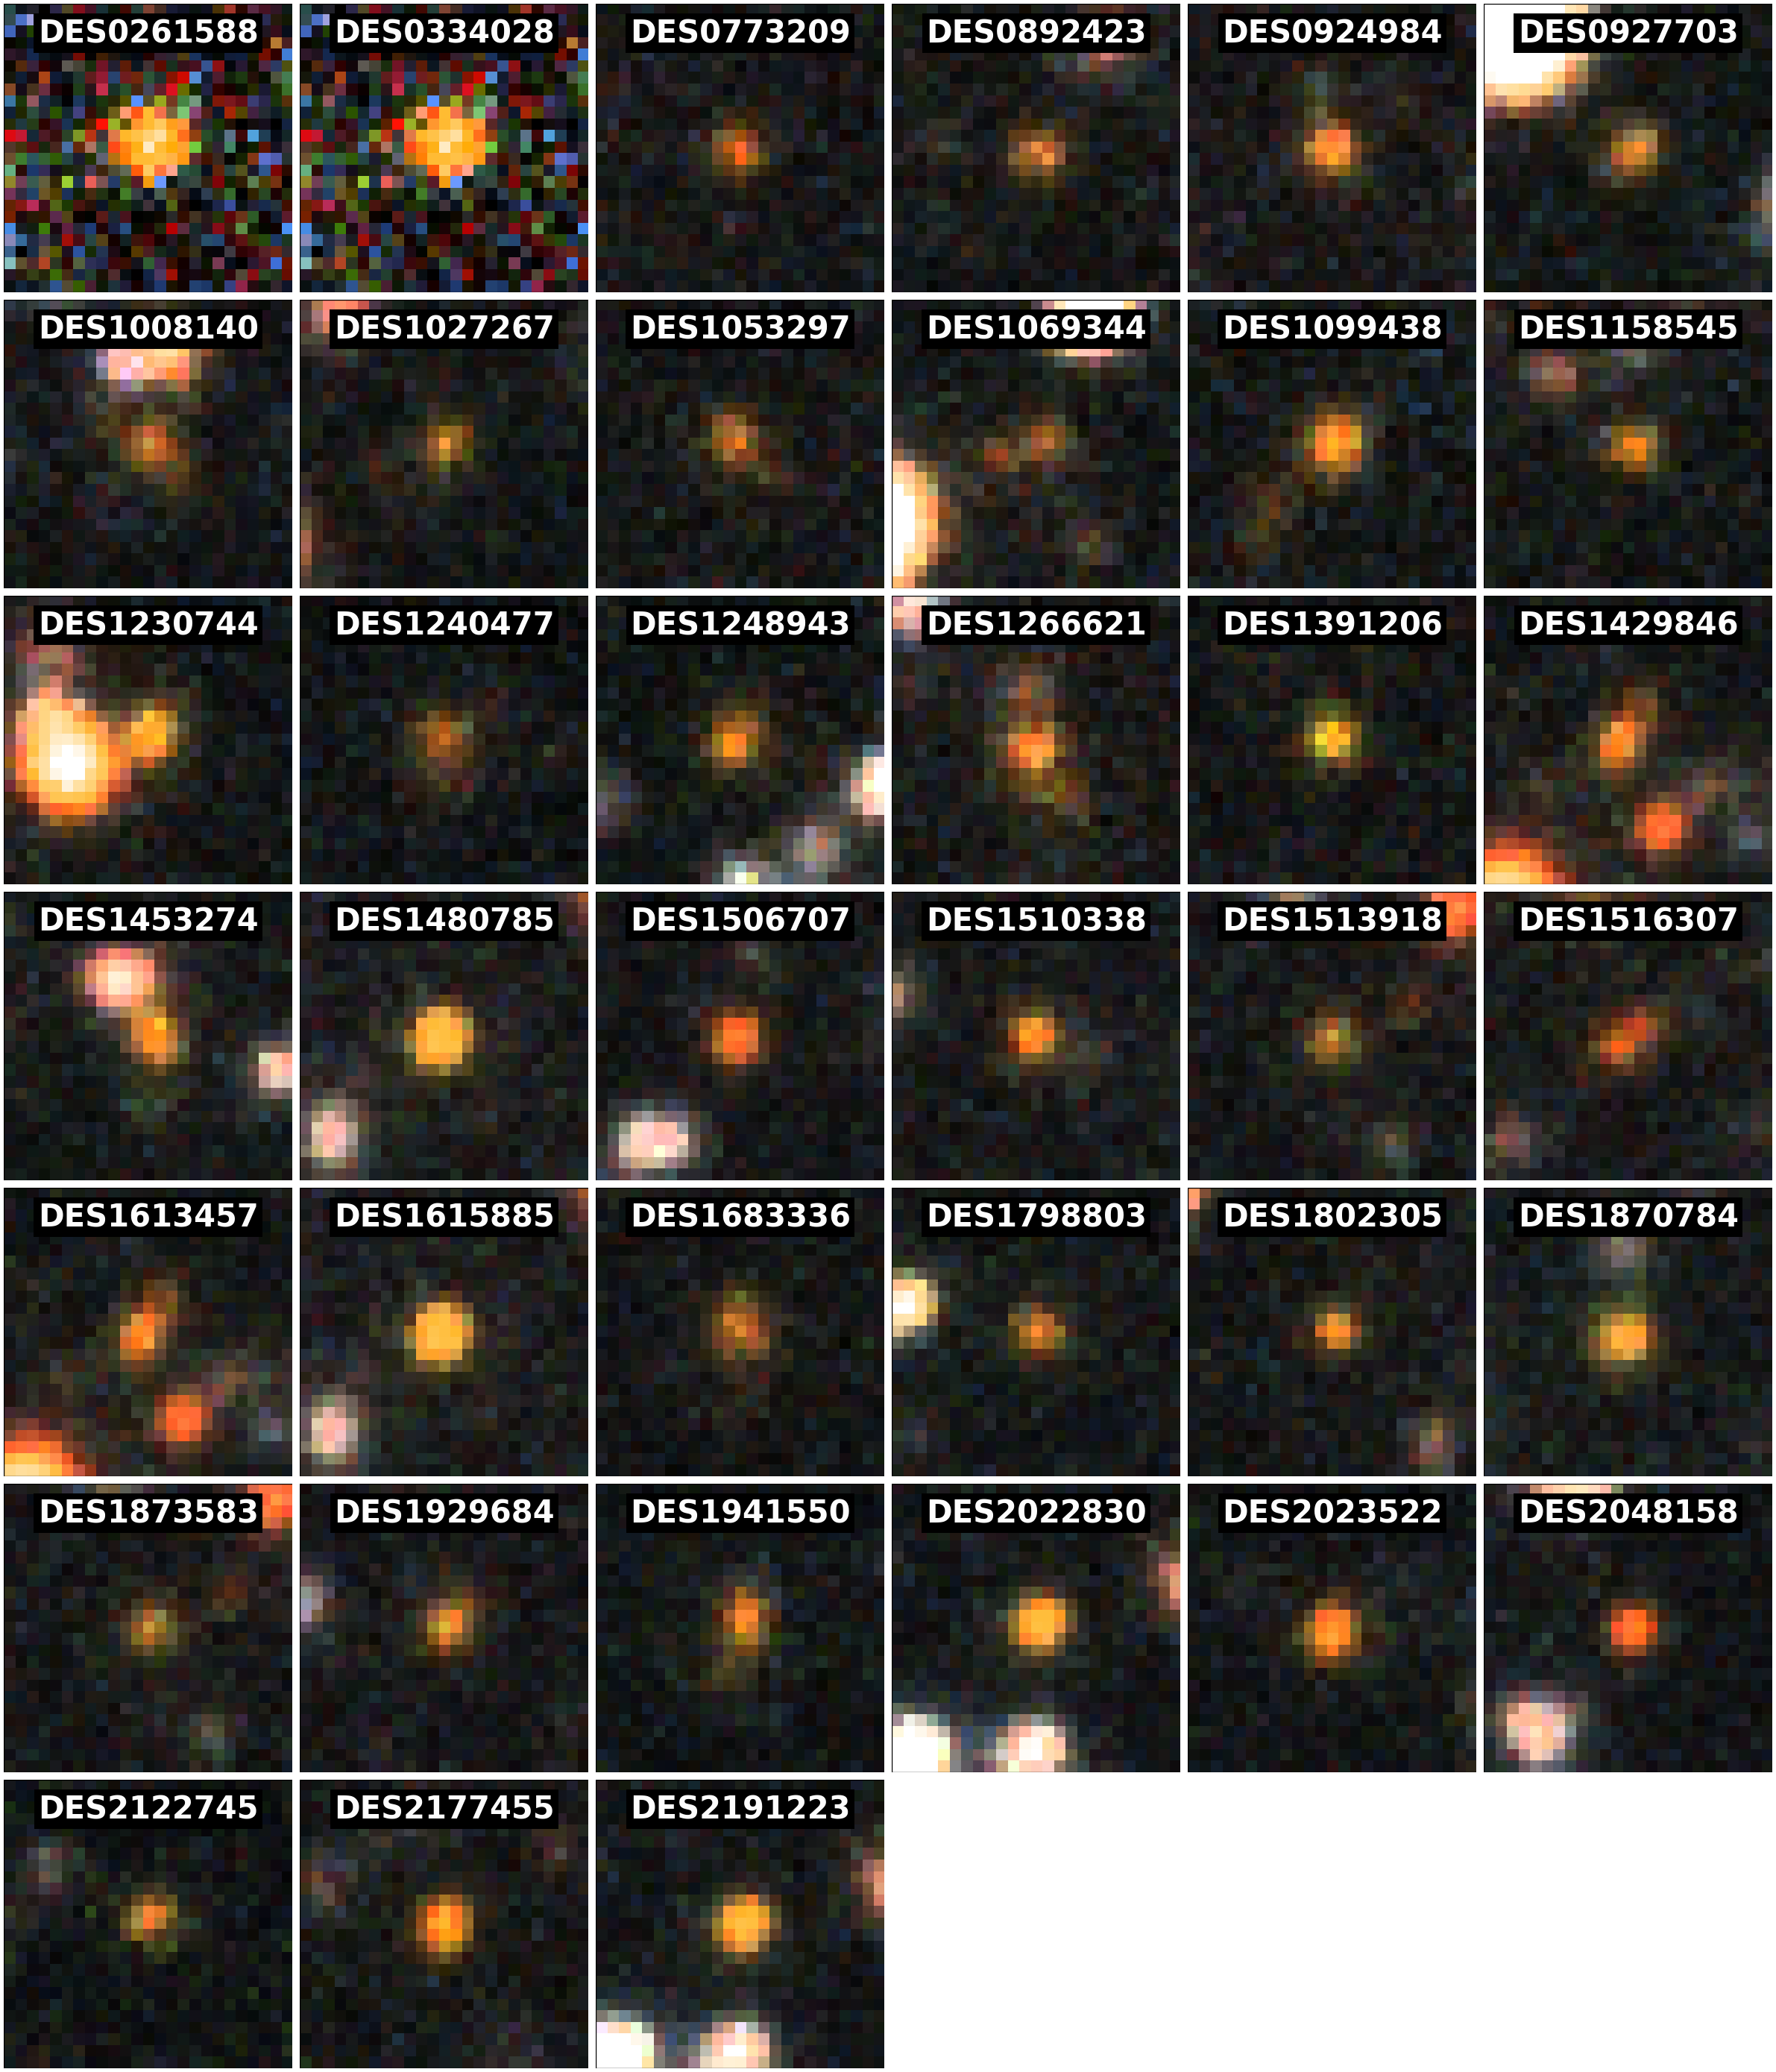
\includegraphics[width=0.95\textwidth]{combine_cutouts_5.png}
\caption[False-colour images of \texorpdfstring{$z\sim5$}{} candidates]{False-colour images of the 39 candidates in the final $z\sim5$ sample. These have been generated from cutouts of the DES $g$-, $r$-, $i$-, and $z$-band data using a custom code created by the author, described in Appendix \ref{appendix:false_colour}. Each image covers an area of $\SI[product-units = repeat]{6.6 x 6.6}{\arcsec}$. It is clear that several pairs of candidates have identical false-colour images; those are duplicates originating from DES tile overlap. It is also interesting to observe that the morphologies of many candidates show signs of extended emission.}
\label{fig:candidates_5}
\end{figure}

\clearpage
\begin{figure}[p]
\centering
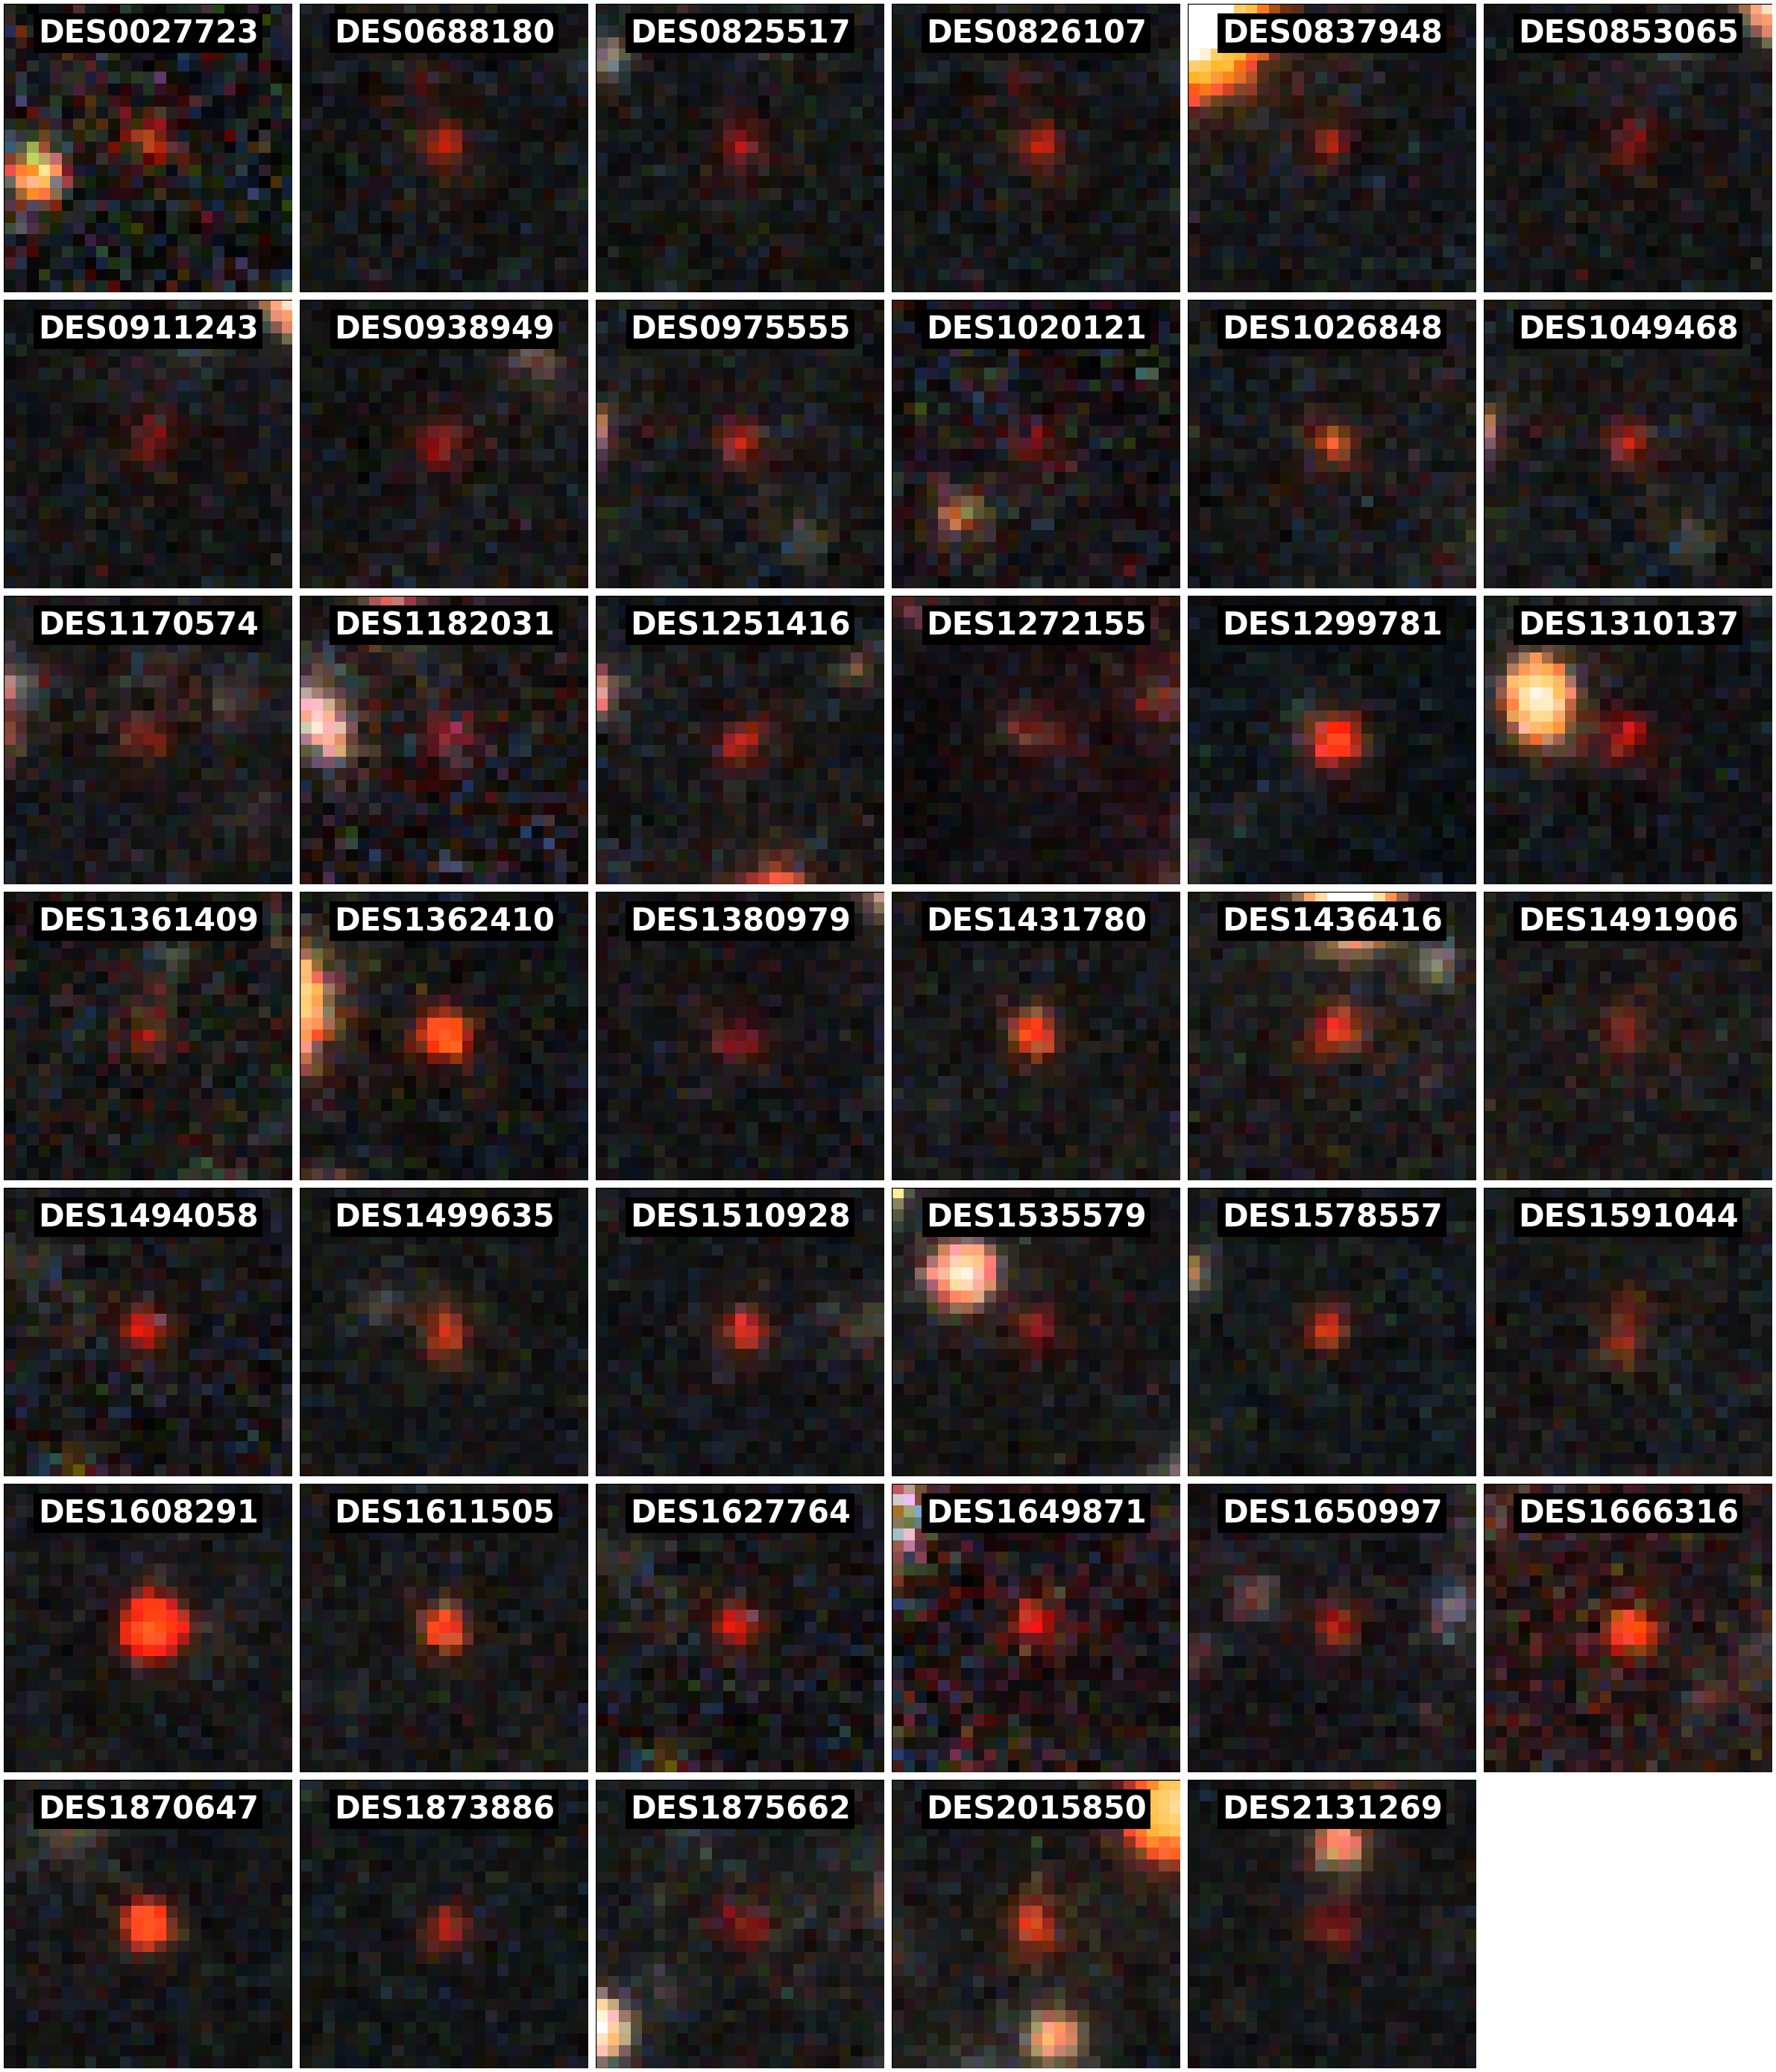
\includegraphics[width=0.95\textwidth]{combine_cutouts_6.png}
\caption[False-colour images of \texorpdfstring{$z\sim6$}{} candidates]{False-colour images of the 41 final  $z\sim6$ candidates, obtained in the same way as for the $z\sim5$ sample in Figure \ref{fig:candidates_5}. The colour calibration and scale are identical, with each cutout covering $\SI[product-units = repeat]{6.6 x 6.6}{\arcsec}$. Similarly to Figure \ref{fig:candidates_5}, some pairs of candidates have identical false-colour images due to the presence of duplicates. Several objects show morphologies indicative of extended emission. It is reassuring to note that the $z\sim6$ candidates generally appear fainter and smaller than their $z\sim5$ counterparts, as would be expected from their greater distances.}
\label{fig:candidates_6}
\end{figure}
\clearpage
}

Now the process for isolating a secure collection of high-redshift candidates has been discussed, the current section focuses on these final candidates in further detail. Table \ref{table:candidates_5} presents the 39 objects in the $z\sim5$ sample, listing their position, photometric redshift and magnitudes in the $r$, $i$, $z$ and $J$ filters. Table \ref{table:candidates_6} lists the corresponding results for the 41 $z\sim6$ candidates. It is worth noting that these samples include duplicates. The total number of unique galaxies is 34 at $z\sim5$, and 36 at $z\sim6$, as both samples contain 5 pairs of duplicates (indicated in the aforementioned tables). The existence of such duplicates is reassuring, because it suggests that the selection method retrieves similar results for flux measurements in tiles with slightly different depths. \par 


False-colour images for the candidates are presented in Figures \ref{fig:candidates_5} and \ref{fig:candidates_6} for the $z\sim5$ and $z\sim6$ samples respectively. These images have been generated using a custom code created by the author, described in detail in Appendix \ref{appendix:false_colour}. It is reassuring to note that several candidates very clearly display extended emission, definitively confirming their status as galaxies. Some of these galaxies even show signs of irregular, ellipsoid, or disk-like shapes. Furthermore, many more (around half the objects in both samples) show a morphology with at least some indications of an extended shape. This is consistent with results from \cite{2015MNRAS.452.1817B} and \cite{2013AJ....145....4W}, who found that over half, but not all, bright $z\sim6$ galaxies are resolved in ground-based imaging (with a slightly lower seeing of \SIrange[range-phrase = \text{--}, range-units = single]{0.7}{0.8}{\arcsec}). \par 


\subsection{Comparison with previous studies}

\subsubsection{Number of expected candidates}\label{subsubsection:expected_number}
It is interesting to estimate the expected number of \DESVIDEO high-redshift candidates based on other research in the literature. In recent years, several authors have found samples of bright $z\gtrsim5$ galaxies. For instance, \cite{2009MNRAS.395.2196M} found 1621 possible\footnote{It must be remarked that this sample was probably not entirely pure. \cite{2009MNRAS.395.2196M} did not exclude objects with a possibility of a secondary solution at low redshift, instead choosing to weight their objects by the redshift probability density function $P(z)$ when computing their luminosity function.} galaxies with magnitudes of $z'_{\mathrm{AB}}< 26.0$ and redshifts of $z>4.5$ over a search area of \SI{0.63}{\sqdeg} with $5\sigma$ depths of $z'_{\mathrm{AB}}\approx26.2$. In a comparable study restricted only to $z\sim6$, \cite{2015MNRAS.452.1817B} searched a deep \SI{1.36}{\sqdeg} region with $5\sigma$ depths of $z'_{\mathrm{AB}}=\numrange[range-phrase = \text{--}, list-units = single]{26.5}{26.8}$, finding 263 candidates with magnitudes of $z'_{\mathrm{AB}}< 26.0$. These two studies suggest that there may be several hundreds, possibly thousands, of high-redshift $z_{\mathrm{AB}}<{26.0}$ objects in the deepest \SI{4}{\sqdeg} of \DESVIDEO data.  However, the search in this thesis is limited to the brightest galaxies with magnitudes of $m_{\mathrm{AB}}< 25.0$, and these luminous sources have been found to be much rarer. Comparable studies in this regime have mainly been conducted at $z\sim6$. The study by \cite{2015MNRAS.452.1817B} found nine bright $z'< 25.0$ candidates in their \SI{1.65}{\sqdeg} search area (situated within the COSMOS and SDXS fields). These candidates, selected via photometric redshifts, span a redshift range of $5.7 <  z <  6.3$. For a \SI{0.29}{\sqdeg} sub-region\footnote{\cite{2015MNRAS.452.1817B} refer to this area as the ULTRAVISTA/COSMOS DR1 region. This region has shallower near-IR data than the other \SI{1.36}{\sqdeg} of their footprint, but has identical $z'_{\mathrm{AB}}= \numrange[range-phrase = \text{--}, list-units = single]{26.5}{26.8}$ limiting magnitudes.} the authors also reported three $z'< 25.0$ galaxies when they imposed $5.5 <  z <  6.5$ limits identical to those used in this thesis. \cite{2013AJ....145....4W} conducted another study that found 14 $z\approx6$ candidate Lyman-break galaxies with magnitudes of $z'< 25.0$ in the four CFHTLS Deep Fields. Their search covered an area of \SI{4}{\sqdeg} with a $5\sigma$ depth of $z'\approx26.5$, and it made use of colour-colour selection criteria, which were most sensitive to galaxies in the range $5.7< z< 6.0$. \par 

%When they imposed $5.5 <  z <  6.5$ limits identical to those used in this thesis, the authors reported three $z'< 25.0$ galaxies for a \SI{0.29}{\sqdeg} sub-region\footnote{\cite{2015MNRAS.452.1817B} refer to this area as the ULTRAVISTA/COSMOS DR1 region. This part has shallower near-IR data than the rest of their \SI{1.36}{\sqdeg} footprint, but has identical $z'_{\mathrm{AB}}= \numrange[range-phrase = \text{--}, list-units = single]{26.5}{26.8}$ limiting magnitudes.}. 

The samples from \cite{2015MNRAS.452.1817B} and \cite{2013AJ....145....4W} can be used to extrapolate the rough number of expected \DESVIDEO $z\sim6$ galaxies. For this it is necessary to know the effective search area, which was measured to be \SI{4.9}{\sqdeg} as previously described in Section \ref{subsubsection:mag_cut}. Using this quantity, the numbers from previous studies were then simply scaled by area to obtain the estimated number of \DESVIDEO catalogues. Those calculations produced an expected total of 27 $z\sim6$ candidates based on the \cite{2015MNRAS.452.1817B} study, and a lower estimate of 17 from \cite{2013AJ....145....4W}. \par

%For this it is necessary to know the effective search area, which was previously introduced in Section \ref{subsubsection:mag_cut}, where it was stated that it is equal to \SI{4.9}{\sqdeg}. 

Clearly, both these values are smaller than the actual \DESVIDEO total of 36 unique candidates. There are several possible explanations for this. Firstly, the \cite{2013AJ....145....4W} estimate of 17 is likely too low, as \cite{2015MNRAS.452.1817B} demonstrated that the \cite{2013AJ....145....4W} selection method excluded many genuine LBGs (possibly by as much as a factor of \numrange{3}{6}). Additionally, both studies restricted their final estimates to a narrower redshift range than \DESVIDEO, so their projected number counts are inherently expected to be lower than those in this thesis. To emphasise this point, if one considers only the \SI{0.29}{\sqdeg} region where \cite{2015MNRAS.452.1817B} quoted three objects within the \DESVIDEO range of $5.5 <  z <  6.5$, the number of estimated candidates rises to 51 --- a little more than were found in this thesis. A further factor is that the number counts and search area in the  \cite{2015MNRAS.452.1817B} sample are small, which makes any extrapolations from their numbers strongly susceptible to random chance, both from selection effects\footnote{It is certainly possible that the photo-zs computations or star-galaxy separation by \cite{2015MNRAS.452.1817B} happened to exclude a few real sources, or that uncertainties in the photometry caused some of their magnitude measurement to be just over $z'=25.0$.} and from variations in the underlying number of actual bright $z\sim6$ galaxies in the fields. Finally, another possible factor may be cosmic variance, although this is prima facie unlikely given the fields in question. The studies by \cite{2013AJ....145....4W} and \cite{2015MNRAS.452.1817B} both include the COSMOS field, which according to either study contains an overdensity of galaxies at $z\sim6$. The \DESVIDEO sample, on the other hand, contains a roughly equal number of objects in the equally-sized\footnote{The effective area in both these fields is approximately equal, and largely corresponds to the deep regions in Figures \ref{fig:depth_xmm} and \ref{fig:depth_cdfs}.} XMM-LSS and CDF-S fields. In the former region, which is also within the \cite{2013AJ....145....4W} search area, \cite{2013AJ....145....4W} found 8 candidates --- similar to the number of objects in their other three fields apart from COSMOS. This implies that none of the \DESVIDEO footprint is likely to be particularly overdense. It is nevertheless possible that cosmic variance did contribute to why the \cite{2015MNRAS.452.1817B} estimate falls below \DESVIDEO. Their paper raised the possibility that the SDXS field (which supplied 45\% of their footprint) may be underpopulated around $z\approx5.7$, which could cause their estimate to be biased slightly low. All things considered, all the mitigating factors in this paragraph suggest that there are several highly plausible reasons why the candidate estimates from previous studies have come out low, which means that these comparisons provide no reason to believe that the \DESVIDEO sample is substantially too large. Consequently, there is no compelling evidence for significant contamination within the sample presented in this thesis. \par 




\subsubsection{Comparison with \texorpdfstring{\cite{2013AJ....145....4W}}{TEXT}}\label{subsubsection:willott_compare}
Conveniently, as mentioned previously, the imaging used by \cite{2013AJ....145....4W} partially overlaps with the \DESVIDEO footprint in the XMM-LSS field. It is therefore interesting to compare their candidates to the $z\sim6$ sample in this thesis. Their selection method used a both a different dataset (optical imaging from the CFHTLS-Deep and near-IR data from an earlier VIDEO release) and a different selection method (based on colour-colour cuts instead of photometric redshifts). Even though most of the candidates in their sample are not spectroscopically confirmed, the \cite{2013AJ....145....4W} objects can therefore be used as an independent means to verify the candidates in this thesis.  \par

Out of the 40 $z\sim6$ Lyman-break candidates found by \cite{2013AJ....145....4W}, eight are located within the \DESVIDEO footprint. Of these eight objects, six unique sources exist in the \DESVIDEO catalogue (WMH2, WMH3, WMH4, WMH5, WMH6, WMH8). The two others, WMH1 and WMH7, are too faint in the $r+i+z$ detection image to be included in the DESDM catalogues, so they are not present in the \DESVIDEO tables. WMH2 is found twice in the \DESVIDEO data, as it is a duplicate that was observed in both the xmm2 and xmm3 VIDEO tiles. \par 


Of the six unique common candidates, only three (WMH2, WMH3 and WMH5) are brighter than the $z_{\mathrm{AB}}< 25.0$ magnitude limit imposed in Equation \ref{eqn:mag_cuts}. It is reassuring to note that all three of these bright objects appear in the final \DESVIDEO candidate sample. Especially encouraging is the fact that this includes WMH5, which was spectroscopically confirmed to be a high-redshift galaxy at $z_{\mathrm{spec}}=6.068$. Moreover, both duplicate instances of WMH2 passed the selection criteria, confirming that the VIDEO photometry in both the xmm2 and xmm3 tiles is sufficient in quality to ascertain its high-redshift status. The \DESVIDEO candidates that correspond to a \cite{2013AJ....145....4W} object are flagged in Table \ref{table:candidates_6}. \par

The remaining three objects (WMH4, WMH6 and WMH8) were not included in the \DESVIDEO sample due to their faint magnitudes. Besides, WMH6 was also assigned a low \DESVIDEO redshift of $z_{\mathrm{phot}}=0.8$, despite it being spectroscopically confirmed at $z_{\mathrm{spec}}=5.645$. This suggests that the selection method in this thesis is indeed less effective in the faint $z_{\mathrm{AB}}>25.0$ regime, and that it is appropriate to impose this magnitude limit. Nevertheless, WMH4 and WMH8 did get assigned \DESVIDEO photometric redshifts of $z_{\mathrm{phot}}=6.1$ and $z_{\mathrm{phot}}=6.0$ respectively, suggesting that the photo-z method in this thesis does retrieve accurate results for some faint sources at (presumed) high redshifts. Furthermore, these two candidates also pass all the other selection criteria in both rounds of Section \ref{section:selection_criteria}, which means that they would have made it into the final sample were it not for the magnitude limit. \par

The conclusion of the comparison in this section is highly encouraging ---  the fact that all three bright \cite{2013AJ....145....4W} galaxies (including the spectroscopically confirmed WMH5) were retrieved as high-redshift candidates provides additional confidence in the selection method used in this thesis. Furthermore, the good performance for 2 out of 3 of the fainter objects is also encouraging. Thirdly, the two \DESVIDEO candidates that correspond to the WMH2 and WMH3 candidates are very likely to be true high-redshift galaxies, as they have independently been found via both the \cite{2013AJ....145....4W} colour-cuts and the photmetric redshift method used in this thesis. \par 




\section{Attempted spectroscopic follow-up}\label{subsection:spectroscopic_confirmation}
%Despite the confidence in the final sample as indicated by the colour chart, it would be good to obtain definite verification of the selection method via spectroscopic redshifts. 

Despite the good level of confidence in the search strategy employed in this thesis, spectroscopic redshifts constitute the only way of confirming the high-redshift status of candidates with certainty. Therefore, the author attempted to obtain spectra for some of the most promising \DESVIDEO candidates. Observing time for this spectroscopic follow-up was kindly secured on the Large Binocular Telescope (LBT) via Paul Martini, who volunteered to observe two candidates on the Multi Object Double Spectrographs (MODS; \citealt{2010SPIE.7735E..0AP}). This instrument also facilitated the observation of a third $z\sim6$ candidate close to one of the original candidates, thanks to its large field of view and capacity to observe multiple objects at once. All in all, candidates DES0938949 (WMH3;  $z_{\mathrm{phot}}=6.07$), and DES1361409 + DES1362410 (observed simultaneously; $z_{\mathrm{phot}}=5.68$ and $z_{\mathrm{phot}}=5.79$ respectively) were submitted for spectroscopic follow-up and observed in October 2016. Unfortunately, the observations yielded no useful spectra, most likely due to bad weather conditions. Further spectroscopic follow-up is therefore highly recommended as an objective for future research. \par 


